\chapter[Introdução]{Introdução}

\section{Contexto}
A tecnologia tem vindo a evoluir rapidamente e, com isto, nota-se o surgimento de
diversos desafios. Um destes desafios é a falta de programadores que possuam competências 
e qualificação necessárias para solucionar os mais diversos problemas presentes nos mais
variados projetos. Este fato está relacionado com a metodologia adotada no ensino de
programação e também com a falta de motivação por parte dos estudantes \cite{7975788}.
\citeonline{inproceedings} afirmam que, uma das razões de os alunos não absorverem eficientemente
os conceitos relacionados à programação se dá pela falta de concentração e motivação dos mesmos frente
a exposição destes conteúdos na forma tradicional.

\citeonline{funcional} destaca que a aprendizagem dos conceitos e mecanismos envolvidos na construção de programas não é
trivial, uma vez que requer a utilização de raciocínio na sua forma mais abstrata. Um dos problemas mais comuns segundo os autores
são: dificuldades no entendimento de comandos, sintaxe dos comandos, dificuldades em entender os resultados da execução de um determinado 
comando pela máquina, dificuldades em dar os primeiros passos relativos ao estudo de programação entre outros.

\citeonline{ambap} diz que, em geral, os alunos têm grandes dificuldades em compreender e aplicar os conceitos relativos à programação . Uma das grandes 
dificuldades está relacionada a problemas de compreensão e aplicação de noções básicas, como por exemplo o uso de estruturas de controle e estruturas
condicionais.

Dificuldades como estas apresentadas, encorajam o desenvolvimento de soluções que auxiliem no ensino e aprendizagem de programação de forma diferente ao
atual modelo de ensino. Diversas abordagens de ensino são estudadas para facilitar o aprendizado dos alunos, algumas delas são:
gamificação, programação imperativa, programação funcional e etc. Neste trabalho, será abordado o uso da gamificação em uma ferramenta
de apoio ao ensino e aprendizagem de programação a ser desenvolvida com base na identificação de requisitos a partir da interação com ex alunos
e alunos atuais da disciplina de Algoritmos de Programação de Computadores, ofertada pela Universidade de Brasília, campus Gama.

Segundo \citeonline{6624228}, jogos bem projetados representam bons motivadores, uma vez que passa a sensação de satisfação
e recompensa fazendo com que os jogadores persistam e fiquem engajados em realizar sua missões. Neste contexto, este poder
motivacional dos jogos, passou a ser utilizado em outros contextos que não estão relacionados diretamente aos jogos, uma prática 
conhecida atualmente como Gamificação do inglês \textit{gamification} {\itshape}.

Para \citeonline{Deterding:2011:GDE:2181037.2181040}, o termo gamificação pode ser definido como a utilização de elementos e mecânica de 
jogos em contextos não relacionados a jogos. De acordo com \citeonline{Brazil} a utilização destes elementos tornam tarefas reais em atividades
mais atrativas e lúdicas e, consequentemente, aumentam a motivação e engajamento. Há uma grande variedade de ambientes que possuem 
elementos semelhantes a características de jogos, muitos deles contendo: sistema de pontuação, feedbacks constantes e 
etc \cite{6624228}. São exemplos de ambientes com características semelhantes a de jogos: Uri, Datacamp, Edx entre outras.

A aprendizagem baseada na gamificação, preocupa-se em utilizar de mecanismos de jogos não para o entretenimento,
mas para o ensino. Os interessados no campo da gamificação trabalham para identificar o cenário e as condições 
que possam apoiar a integração de jogos aos ambientes de aprendizado. Vários cientistas e estudiosos no campo
da gamificação apontaram uma diversidade de elementos de jogos que permitem que eles sejam utilizados como
ferramentas de apoio ao aprendizado. Por exemplo: os jogos são bastante envolventes \cite{Dickey2005} e motivadores \cite{Prensky:2003:DGL:950566.950596}. Além destas características,
jogos são excelentes fontes para se adquirir experiência que são dificeis de serem fornecidas por meio de instruções tradicionais \cite{Arena2014}.

Os ambientes online gamificados de apoio ao ensino podem fornecer diversas ferramentas, entre elas: classificações, batalhas, fórums de discussões e etc.
De forma a incentivar os usuários a participarem das atividades propostas. 
Durante as competições e batalhas, os estudantes têm a possibilidade de aprender com outros jogadores e comparar suas habilidades, tornando o aprendizado mais
prazeroso \cite{LearningProgramming}. 

\pagebreak

\section{Justificativa}
De acordo com \citeonline{de2009visualg}, a abordagem de ensino tradicional de programação, que é aquela onde o professor apresenta
uma série de conceitos aos alunos e os mesmos têm a tarefa de entender como se aplicam na resolução de problemas,
para a maioria dos estudantes, se revelam muito abstratas.

Em seu trabalho de conclusão de curso pela Universidade de Brasília , campus Gama (FGA), \citeonline{calixto} apresenta uma pesquisa 
baseada nos dados referentes aos índices de aprovação, trancamento e reprovação dos alunos na disciplina de computação básica (atualmente
a disciplina recebe o nome de Algoritmos e Programação de Computadores, ofertada no campus Gama). 

Os dados utilizados por \citeonline{calixto}, são referentes a um total de 60 turmas e 3286 alunos matrículados nas disciplinas de Computação Básica entre
os anos de 2009 e 2013. Segundo o autor, dos 3286 alunos matriculados, 1659 alunos (50,48\%) foram reprovados, 262 alunos (8\%) trancaram
a disciplina e apenas 1364 alunos (41,5\%) obtiveram aprovação. O autor ainda explica que esses resultados, quando comparados à média nacional de 
aprovação de alunos em disciplinas de programação são bem preocupantes, a taxa apresentada como média nacional é de cerca de 67\% de aprovação, ou 
seja, a taxa de aprovação na FGA, é mais de 30\% menor em relação a média apresentada (67\%).

Contando com a cooperação dos funcionários da secretaria da FGA, obteve-se dados atuais referentes às aprovações, reprovações e trancamentos dos
alunos entre os períodos 2017/1 e 2019/1. Ao analisar estes dados, notou-se que do total de alunos matriculados (2225 alunos divididos em 37 turmas) no decorrer
de 5 semestres, 890 alunos (40\%) foram reprovados, 112 alunos realizaram o trancamento (5\%) e apenas 1223 alunos foram aprovados (54,96\%). Estes dados são preocupantes 
e demonstram a atual situação do aprendizado dos alunos na disciplina de Algoritmos e Programação de Computadores na FGA.

Um estudo realizado pela Universidade Federal da Paraíba (UFPB) que analisou por seis períodos 
acadêmicos os índices de reprovação na disciplina de Introdução à programação, apontou que 
em nenhum dos seis períodos analisados houvera um índice de aprovação superior a 34\%. Além disso,
os índices de reprovação e trancamento da disciplina giraram em torno dos 64\% e 6\% respectivamente \cite{SBIE6739}.

Um outro estudo, realizado na Faculdade de Educação Tecnológica do Estado do Rio de Janeiro (FAETERJ-Paracambi) por \citeonline{vieira2015dificuldades}, 
envolvendo 663 alunos da disciplina de Algoritmos 1 mostrou que, destes alunos, apenas 511 cursaram a disciplina 
até o final, ou seja, cerca de 152 alunos desistiram da disciplina. Do total restante (511), apenas 30\% foram
diretamente aprovados (cerca de 153 alunos), 40\% foram reprovados diretamente (204 alunos) e 30\% foram para o exame final (recuperação, 153).
Dos 153 alunos que foram para a recuperação, apenas 55\% foram aprovados (84 alunos), nota-se então que, dos 663 alunos que
foram matriculados na disciplina, apenas  288 alunos foram aprovados ao seu término, cerca de 43\%.

\section{Problema}
Nas seções anteriores, apresentou-se alguns estudos realizados a respeito da situação atual do ensino e aprendizagem
de programação em matérias introdutórias, a partir destes panoramas, o presente trabalho visa responder a seguinte temática
de pesquisa:
Como desenvolver uma ferramenta gamificada para auxiliar o ensino e aprendizagem de programação?
 
\section{Objetivos}
Tendo sido apresentado o contexto e problema, o objetivo geral do presente trabalho é
desenvolver uma ferramenta que auxilie professores e estudantes no processo de ensino e aprendizagem
de linguagens de programação em cursos de engenharias. 

Para alcançar o objetivo geral, foram definidos os seguintes objetivos específicos:
\begin{itemize}
	\item Identificação dos requisitos necessários para a construção da ferramenta;
	\item Desenvolvimento da ferramenta gamificada;
	\item Definição do método de coleta de dados a respeito da utilização da ferramenta pelos usuários;
	\item Análise dos dados a respeito da experiência de uso.
\end{itemize}

\chapter[Referencial Teórico]{Referencial Teórico}

\section{Aprendizagem de programação}
De acordo com \citeonline{KOLIVER}, disciplinas introdutórias de programação são, em sua maioria, problemáticas e costumam apresentar
altos índices de desistência e reprovações. Um dos motivos para tal ocorrência se dá pela falta de preparo que se espera que alunos
ingressantes nestas disciplinas possuam.

Disciplina de algoritmos são normalmente oferecidas no início da grade curricular dos cursos. Isso faz com que a maioria dos alunos
cursantes sejam calouros que ainda estão acostumados com a forma ``mecanisada'' de ensino que os habituam a somente aplicar fórmulas 
sem qualquer tipo de análise mais profunda dos problemas \cite{KOLIVER}.

De acordo com \citeonline{Borges}, o modo tradicional de ensino (figura \ref{figura4}) não é suficiente para motivar os alunos a se
interessarem por disciplinas de programação. Não fica claro para a maioria dos alunos, principalmente para aqueles
não possuem nenhum tipo de conhecimento em informática, a importância de certos conteúdos.

\begin{figure}[h]
	\centering
	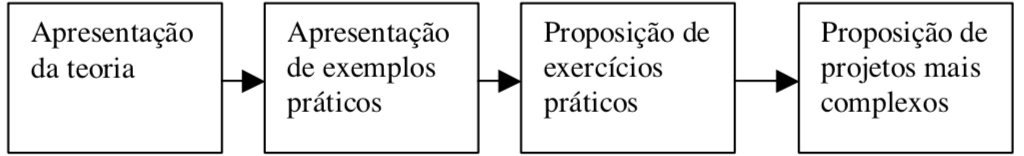
\includegraphics[keepaspectratio=true,scale=0.34]{figuras/modoTradicional.png}
	\caption{Sequência de passos típicos na apresentação de uma disciplina}
	Fonte: \cite{Borges}
	\label{figura4}
\end{figure}

Ao se apresentar uma nova liguagem de programação, é comum as aulas serem realizadas em laboratórios com
recursos computacionais. Apesar dessas aulas apresentarem um formato diferenciado em relação ao modo tradicional,
os professores não exploram a diversidade dos equipamentos disponíveis com práticas que apoiem o desenvolvimento 
de habilidades por parte dos estudantes \cite{Borges}.

\section{Gamificação}
Jogos são uma construção humana que envolvem em seu contexto fatores sociais, culturais e econômicos \cite{EaDF440}.
Como apresentado no livro ``Gamificação na Educação'' por \citeonline{da2014gamificaccao}, a interação com \textit{games}, apesar
dos custos altos dos consoles, foram ocupando cada vez mais o tempo das pessoas que notaram que os jogos poderiam ser boas fontes
de prazer e entretenimento.

O notável crescimento do mercado dos \textit{games} tem atraido diferentes olhares de estudiosos que se dedicam ao estudo de seu
uso na educação, comunicação, marketing, psicologia, computação, entre outras áreas \cite{da2014gamificaccao}.

O termo gamificação, segundo \citeonline{da2014gamificaccao}, consiste na utilização de elementos de jogos em 
atividades que por natureza de sua criação não são jogos. \citeonline{raposo2016desafio} dizem que o objetivo da gamificação, consiste em resolver
problemas práticos ou despertar interesse e engajar um público específico para a realização de uma determinada
atividade. 

Para \citeonline{chou2017actionable}, a gamificação é uma arte que é capaz de derivar elementos divertidos e envolventes encontrados em jogos e utiliza-los
em outras atividades. Para o autor, o foco deve estar centrado no ser humano e na sua motivação.

\subsection{Gamificação na Educação}
Embora o termo gamificação tenha sido apresentado pela primeira vez em 2010, a idéia de se utilizar
elementos de jogos em atividades que não são jogos, tem sido utilizado há muito tempo. Na educação
de crianças, por exemplo, as mesmas podiam ter seus esforços e trabalhos reconhecidos por meio
de estrelinhas ou outros tipos de recompensas dadas por seus educadores, como explica \citeonline{da2014gamificaccao}.

De acordo com \citeonline{da2014gamificaccao}, no Brasil existem diversas instituições públicas e privadas que apoiam o desenvolvimento e uso de ambientes
gamificados. A exemplo disto, o Ministério da Educação visa fornecer suporte para o ambiente gamificado de apoio ao ensino \textit{Geekie games} que possibilita
aos estudantes se prepararem para o Exame Nacional de Ensino Médio (ENEM). Os resultados da utilização da ferramenta, segundo \citeonline{da2014gamificaccao}, 
foram considerados positivos e o Ministério da Educação levanta a possibilidade de extender o uso da ferramenta gamificada para outros sistemas de avaliação.

Segundo \citeonline{hammer}, somente a utilização de elementos de jogos no ensino não resolve a falta de empatia no processo de aprendizagem dos alunos
uma vez que a utilização de mecanismos como por exemplo o sistema de pontuação já estão presentes no cotidiano escolar há anos. De acordo com as autoras, 
a utilização de elementos e característica de jogos devem provocar impactos tanto emocionais quanto sociais nos indivíduos para que eles tenham um aprendizado
efetivo. 

\section{\textit{Framework Octalysis}}
No livro \textit{"Actionable Gamification – Beyond Points, Badges, and Leaderboards"}, \citeonline{chou2017actionable} apresenta uma série
de características que, segundo ele, atraem e motivam pessoas a tomarem decisões e a realizarem determinadas atividades.
\citeonline{chou2017actionable} ressalta ainda que essas características estão presentes na maioria dos jogos bem sucedidos.

Ao estudar uma variedade de técnicas de jogos que fazem com que os mesmos sejam tão atraentes, \citeonline{chou2017actionable} notou que estas 
técnicas impulsionam os jogadores de maneiras diferentes. Algumas estimulam os jogadores a permanecerem no jogo por meio da
inspiração e capacitação, outras estimulam por meio da manipulaçãoe e obsessão.

Com o aprofundamento de sua pesquisa e a partir da observação de como as técnicas de jogos influenciam nos jogadores, \citeonline{chou2017actionable} 
propôs uma estrutura de design de gamificação que foi apelidada de  \textit{Framework Octalysis}.

O \textit{Framework Octalysis} une elementos de \textit{design} de jogos com a psicologia objetivando motivar os envolvidos
no processo de gamificação a realizarem determinadas ações. O modelo de \citeonline{chou2017actionable} apresenta oito eixos principais que 
são chamados de \textit{core drives}, cada \textit{core} apresenta características que por sua vez apresentam técnicas que
influenciam diretamente os jogadores. Nas subseções a seguir, é apresentado cada um dos oito \textit{core drives}
definidos por Yu-Kai Chou.

\subsection{Significado épico e chamado}
Significado épico e chamado, segundo \citeonline{chou2017actionable}, é um \textit{core} que provoca a sensação no jogador de que ele está envolvido em algo 
grande e que foi especialmente escolhido para executar uma determinada ação. Ao realizar uma contribuição para a plataforma Wikipedia, por exemplo,
as pessoas acreditam que estão ajudando a proteger e disseminar algo que é maior que elas, o conhecimento humano \cite{chou2017actionable}. O próprio autor relata 
em seu livro a experiência que teve com a criação de uma página na Wikipedia com informações de sua empresa, página criada por ele permaneceu no ar por pouco minutos.
Vários contribuintes da Wikipedia relataram que a página não era significante o suficiente para merecer estar na Wikipedia, vários membros concordaram com
a insignificância da página e, após aproximadamente dez minuto a página foi retirada do ar. Para \citeonline{chou2017actionable}, isso 
ocorreu devido ao fato de as pessoas que constituiam a "comunidade Wikipedia", ao realizarem o trabalho voluntário de inspecionar os conteúdos da plataforma, sentirem
que estão fazendo parte de algo que é maior que elas e que de certa forma estão protegendo o conhecimento humano.

Em seguida são apresentadas algumas técnicas de ``Significado épico e chamado'' segundo \citeonline{chou2017actionable}.
Demais técnicas podem ser apreciadas em seu livro presentes no livro \textit{"Actionable Gamification – Beyond Points, Badges, and Leaderboards"}.

\begin{itemize}
	\item Narrativa: A maioria dos jogos iniciam com uma história que mostra aos jogadores o contexto sobre o qual está
	inserido o jogo e o quão importante o jogador é para solucionar os desafios propostos. Uma das maneiras mais eficazes
	em utilizar este núcleo é por meio de uma narrativa envolvente. 
	\item Herói da humanidade: Em seu livro, \citeonline{chou2017actionable} apresenta exemplos que demonstram a natureza desta
	técnica. A empresa \textit{"Tom's Shoes"}, por exemplo, envia um par de sapatos para uma criança em país de terceiro mundo sempre
	que um de seus clientes realiza um novo pedido. O site \textit{"Free Rice"} doa dez grãos de arroz para cada resposta correta dadas
	para as perguntas educacionais postadas no site. Mecanismos como este, passam a sensação de ``heroismo'' aos envolvidos, fazendo com que 
	os mesmos se sintam motivados em participar das atividades propostas;
	\item Sorte de iniciante;
	\item Criança predestinada;
	\item Almoço grátis;
	\item Elitismo;
	\item Significado superior.

\end{itemize}

\subsection{Desenvolvimento e Conquista}
Desenvolvimento e conquista é o segundo \textit{core} do \textit{framework} e está relacionado à motivação interna de 
cada pessoa em desenvolver suas habilidades e superar desafios. Neste núcleo, o desafio para se conquistar, por exemplo, 
um troféu ou distintivo é muito importante, uma vez que conquistar estes artefatos sem um desafio se torna insignificante.
De acordo com \citeonline{chou2017actionable}, essa é a unidade mais fácil de ser projetada. 

Alguns exemplos de técnicas utilizadas neste \textit{core} são apresentadas em seguida.

\begin{itemize}
	\item Pontos;
	\item Lista de desafios;
	\item Luta contra chefes;
	\item Tutorial passo a passo;
	\item Prêmios;
	\item Barra de progresso;
	\item Medalhas;
	\item Emblemas;
	\item Ranking.
\end{itemize}


\subsection{Empoderamento e feedback}
Empoderamento e feedback é o terceiro \textit{core} e está ligado ao uso de táticas visando promover a realização pessoal
do usuário de forma a aumentar seu potencial. Geralmente é expresso quando os usuários se envolvem em um processo criativo
onde os mesmos descobrem coisas novas e, a partir disso, passam a tentar combinações novas, recebendo \textit{feedbacks}
de acordo com os resultados destas novas combinações.

Alguns exemplos de técnicas utilizadas neste \textit{core} são apresentadas em seguida.

\begin{itemize}
	\item Controle em tempo real;
	\item Desbloqueio de marcos;
	\item Combinações em cadeia;
	\item \textit{Feedback} instantâneo;
	\item \textit{Boosters};
	\item Autonomia;
	\item Percepção de escolhas.
\end{itemize}



\subsection{Propriedade e posse}
Propriedade e posse é o quarto \textit{core}. É onde os usuários são motivados a permanecerem nas atividades por
sentirem que possuem controle sobre alguma coisa. De acordo com \citeonline{chou2017actionable}, quando uma pessoa
sente que tem propriedade sobre alguma coisa, a atitude dela é de querer aumentar e melhorar o que possui. Se uma pessoa
gasta muito tempo personalizando seu avatar, automaticamente sente mais propriedade e controle sobre ele ou quando ela é
recompensada com uma moeda virtual ou bens virtuais, a postura dela é realizar mais atividades objetivando receber
e acumular mais bens.

Alguns exemplos de técnicas utilizadas neste \textit{core} são apresentadas em seguida.

\begin{itemize}
	\item Bens virtuais;
	\item Construir a partir do zero;
	\item Coleções;
	\item Avatares;
	\item Curva de aprendizado;
	\item Proteção;
	\item Monitoramento.
\end{itemize}


\subsection{Influência e relacionamento social}
Influência e relacionamento social é o quinto \textit{core} e envolve todos os elementos e características sociais que 
motivam as pessoas. São alguns destes elementos: aceitação social, competição, feedback social e até inveja. Em seu livro,
\citeonline{chou2017actionable} diz que, quando vemos um amigo que possui uma ótima habilidade em alguma coisa, logo nos sentimos
motivados a alcançar o mesmo. Quando alguém nos fala que alcançou um determinado nível em um jogo, por exemplo, a nossa reação, na maioria das 
vezes, é de querer superar a pessoa e, portanto nos engajamos para realizar tal feito.

Alguns exemplos de técnicas utilizadas neste \textit{core} são apresentadas em seguida.

\begin{itemize}
	\item Amizades;
	\item Reconhecimento social;
	\item Atividades em grupo;
	\item Orientações.
\end{itemize}


\subsection{Escassez e impaciência}
A escassez e a impaciência é o sexto \textit{core} e consiste na urgência de se obter algo só porque é raro, exclusivo ou inatingível. De 
acordo com \citeonline{chou2017actionable}, o facebook, por exemplo, na época em que foi lançado era exclusivo para estudantes de \textit{Harvard}, 
depois foi aberto para outras Universidades de grande prestígio e finalmente, quando aberta para todos os públicos, universitários ou não, 
houve um grande aumento no número de pessoas que queriam participar da rede social pelo simples fato de que anteriormente não podiam.

Alguns exemplos de técnicas utilizadas neste \textit{core} são apresentadas em seguida.

\begin{itemize}
	\item Dinâmica de nomeação;
	\item Intervalos fixos;
	\item \textit{Feedback paciente};
	\item Fossos;
	\item Aceleradores;
	\item Contagem regressiva.
\end{itemize}


\subsection{Imprevisibilidade e curiosidade}
Imprevisibilidade e curiosidade é o sétimo \textit{core} e exige o envolvimento constante, uma vez que não se tem nenhuma previsão
do que acontecerá. \citeonline{chou2017actionable} explica que, quando algo não se enquadra nos nossos ciclos regulares de reconhecimento
de padrões, nosso cérebro entra em ação e passa a focar no inesperado, prendendo nossa atenção ao que pode vir a ocorrer. Yu-Kai Chou explica
ainda que esse é o principal núcleo por trás dos vícios nos jogos de azar.

Alguns exemplos de técnicas utilizadas neste \textit{core} são apresentadas em seguida.

\begin{itemize}
	\item Escolha brilhante;
	\item Mini desafios;
	\item \textit{Easter eggs};
	\item Recompensas aleatórias;
	\item Travessuras;
	\item Maravilha óbvia;
	\item Recompensas repentinas.
\end{itemize}



\subsection{Prevenção e perda}
Prevenção e perda é o oitavo e último \textit{core} do \textit{framework} e está relacionado à motivação em se evitar que algo negativo
aconteça. Exemplo: realizar alguma ação em um jogo para evitar que pontos sejam perdidos por falta de atividade.

Alguns exemplos de técnicas utilizadas neste \textit{core} são apresentadas em seguida.

\begin{itemize}
	\item Perda de progresso;
	\item Preguiça de status Quo;
	\item Carta escarlate;
	\item Sepulturas visuais.
\end{itemize}



\section{Elementos motivacionais: Octógono}
De acordo com \citeonline{chou2017actionable}, tudo o que se faz em relação à gamificação é baseado em um ou mais \textit{core drives}. 
Quando não há nenhum dos oito núcleos, a motivação é zero e nenhuma atividade é realizada.


\subsection{Divisão dos motivadores de acordo com sua natureza}

Cada um dos oito \textit{core drives} possuem naturezas diferentes. Alguns fazem os usuários se sentirem poderosos mas não criam a 
sensação de urgência, outros já criam essa sensação nos usuários, além de obsessão e vício. Como resultado destas diferentes características,
as oito unidades do \textit{framework} são mapeadas em um octógono onde a posição de cada um determina a natureza da motivação. Na figura \ref{octogono1}
é apresentado a distribuição de cada \textit{core drive} no octógono.

\begin{figure}[h]
	\centering
	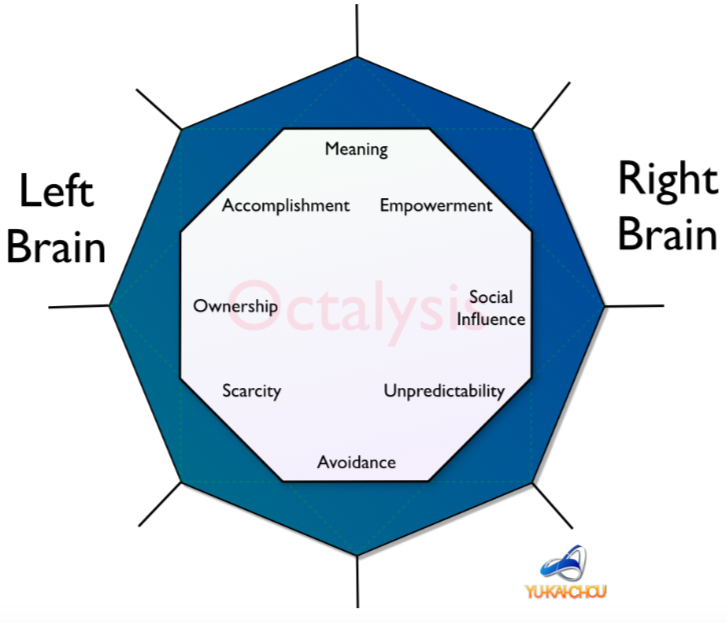
\includegraphics[keepaspectratio=true,scale=0.34]{figuras/brain.png}
	\caption{Divisão do octógono}
	Fonte: \cite{chou2017actionable}
	\label{octogono1}
\end{figure}

A estrutura do \textit{Octalysis} é organizada de forma que os núcleos relacionados à criatividade, auto expressão e dinâmica social são
representados dos lado direito do octógono ("\textit{Right Brain}"). Os núcleos relacionados à logica, pensamento analítico e propriedade são representados graficamente
no lado esquerdo (\textit{"Left Brain"}). É importante ressaltar que ``\textit{Right Brain}'' e \textit{``Left Brain''} não são literais no que se refere
à regiões do cérebro humano, a utilização destes termos é apenas um simbolismo.

\subsection{Gamificação \textit{White Hat} e \textit{Black Hat}}

Uma característica importante na representação dos núcleos motivacionais dentro do octógono é a forma como eles estão agrupados em relação ao impacto
que causam sobre os participantes. Os núcleos localizados na parte superior do octógono são considerados ``motivadores positivos'' enquanto os núcleos localizados
na parte inferior do octógono são considerados "motivadores negativos". Os \textit{cores} apresentados na parte superior são chamados de \textit{"White hat"} e os inferiores
são conhecidos como \textit{"Black hat"}. Na figura \ref{octogono} é apresentado a divisão dos núcleos levando em consideração o tipo de motivador em que cada um
é classificado.

\begin{figure}[h]
	\centering
	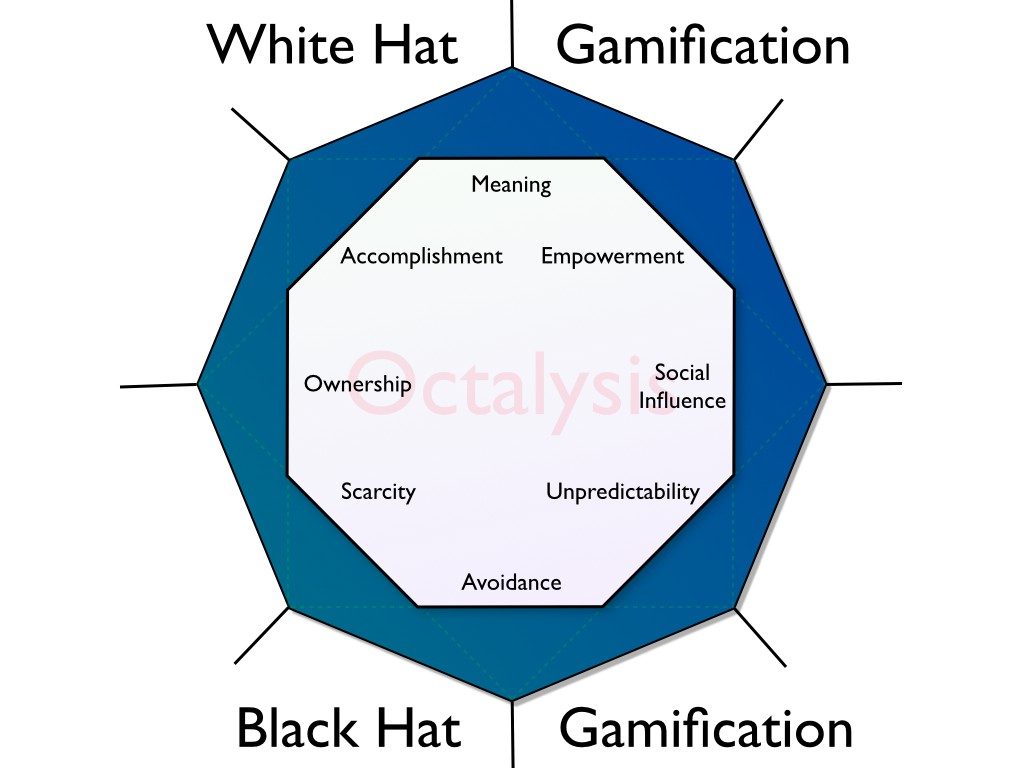
\includegraphics[keepaspectratio=true,scale=0.28]{figuras/octogono.jpg}
	\caption{Gamificação \textit{White hat} e \textit{Black hat}}
	Fonte: \cite{chou2017actionable}
	\label{octogono}
\end{figure}

\citeonline{chou2017actionable} apresenta um exemplo do que vem a ser os núcleos \textit{"White hat"} e \textit{"Black hat"}. Se algo é envolvente
por permitir que se expresse a criatividade, faz com que os indivíduos envolvidos se sintam bem sucedidos e poderosos, com certeza há um \textit{core} 
\textit{"White hat"} sendo utilizado. Por outro lado, se os envolvidos realizam determinadas ações por não saber o que acontecerá logo em seguida ou está
constantemente com medo que algo ruim possa acontecer, neste caso, há um \textit{core} \textit{"Black hat"} sendo utilizado.

Como apresentado por \citeonline{chou2017actionable}, não é porque alguma coisa é categorizada como \textit{"black"} que ela seja ruim. Se utilizadas
corretamente podem gerar resultados saudáveis e positivos. De acordo com \citeonline{chou2017actionable}, um profissional de gamificação deve sempre considerar
todos os \textit{core drive} objetivando obter resultados positivos e produtivos.


\subsection{Níveis \textit{Octalysis}}

O \textit{framework Octalysis} é dividido em vários níveis que, quanto mais alto forem, mais domínio por parte do ``gamificador'' é requerido \cite{chou2017actionable}.
Nas subseções que se seguem, são apresentadas as características relacionadas aos três primeiros níveis do \textit{octalysis}.

\subsubsection{Nível 1}
Para ser aplicado, este nível deve levar em consideração pontos fortes e fracos de vários produtos, este primeiro método permite identificar
que tipos de motivação são fracas para que se possa introduzir novas melhorias \cite{chou2017actionable}.

O segundo método consiste na criação de uma nova experiência baseada nos \textit{core drives} através de um processo sistemático.

Como citado em seções anteriores, neste nível sempre há a necessidade de se utilizar ao menos um \textit{core drive}, caso não seja utilizado nenhum
dos oito núcleos, a motivação é zero e nenhum progresso relativo à gamificação é alcançado \cite{chou2017actionable}.

\subsubsection{Nível 2}
Este nível envolve todas as quatro fases da jornada de um jogador. Em seguida são apresentadas cada uma das quatro fases, bem como suas características.

\begin{itemize}
	\item Descoberta: Experimentações e ganhos de experiências por parte dos jogadores;
	\item Entrada: Aprendizado das regras e ferramentas necessárias para jogar o \textit{game}.
	\item Dia a dia: Jornada regular de ações e comportamentos que os jogadores devem realizar para completar os objetivos;
	\item Fim de jogo: Manter os jogadores motivados a continuarem jogando.
	
\end{itemize}

\citeonline{chou2017actionable} argumenta que o motivo pelo qual as pessoas utilizam um produto no dia 1 muitas das vezes é bastante diferente do
motivo de uso no dia 100. Por este motivo, é importante se planejar cada uma das quatro fases envolvidas na trajetória dos jogadores. Caso não haja nenhum
\textit{core drive} envolvido em alguma das fases, o jogador não possui uma razão para passar para a próxima fase e ele simplesmente desiste.

\begin{figure}[h]
	\centering
	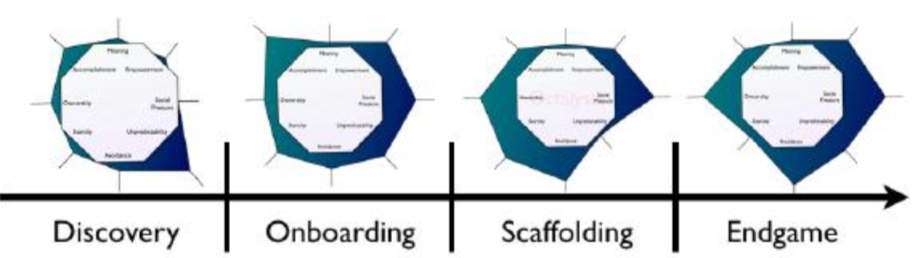
\includegraphics[keepaspectratio=true,scale=0.48]{figuras/fasesjornada.png}
	\caption{As fases da jornada de um jogador.}
	Fonte: \cite{chou2017actionable}
	\label{fasesjornada}
\end{figure}

Observando a figura \ref{fasesjornada}, é possível notar os \textit{core drives} mais proeminentes durante cada fase de experiência da jornada
dos jogadores.

\subsubsection{Nível 3}
Este nível está relacionado com a identificação dos perfis de jogadores e como eles se comportam quando estão envolvidos em jogos. Mesmo que seja
praticamente impossível, este nível permite aos projetistas de gamificação buscar atender as necessidades e motivações dos mais diferentes perfis.

\subsubsubsection{\textit{Design} de gamificação: Octalysis e Bartle}

Embora a classificação dos perfis dos jogadores seja uma proposta criada por \citeonline{bartle1996hearts}, \citeonline{chou2017actionable} apresenta um modelo
que une os perfis apresentados por Bartle com os \textit{core drives} apresentados no \textit{framework Octalysis} de forma a criar um \textit{design} de gamificação
mais apropriado para cada tipo de perfil.

Como apresentado por \citeonline{gamification} no livro ``Gamification: reinventando empresas a partir de jogos'' e com base nos estudos de \citeonline{bartle1996hearts}, 
existem quatro perfis de jogadores que possuem características e comportamentos específicos quando envolvidos em jogos. Cada um destes quatro perfis são apresentados na
subseção a seguir.

\subsubsection{Perfis de Jogadores}

\subsubsubsection{Predadores (\textit{Killers})}
São aqueles jogadores que participam de uma competição pelo prazer de derrotar os adversários. O objetivo desse tipo de jogador é ser o melhor, não 
se importam com o que está em disputa. Possuem comportamentos agressivos e focados em conquistar a posição de liderança. Seus desejos de liderança se 
sobrepõem à cooperação.

\subsubsubsection{Realizadores (\textit{Achievers})}
A motivação destes jogadores consiste na realização de todas as atividades que o jogo apresenta. Esses jogadores apreciam a sensação constante
de vitória mesmo que os objetivos a serem alcançados não sejam tão relevantes ou significativos. Atuam de maneira cordialmente competitiva, mesmo que não estejam
liderando algum placar. São caracterizados por se destacarem dos demais jogadores de maneira leal, isto é, por meio de suas próprias conquistas.

\subsubsubsection{Exploradores (\textit{Explorers})}
Este é um grupo que se caracteriza pela busca e interesse em desvendar todas as possibilidades dos jogos. São indivíduos curiosos que se dedicam em estudar
e desenvolver habilidade que lhes permitam solucionar os mais diversos desafios. Para este tipo de perfil, a trejetória é mais importante que a conquista.

\subsubsubsection{Socializadores (\textit{Socializers})}
São, no geral, os indivíduos que enxergam o contato com jogos como um meio de interação social. Mais significativo que atingir os objetivos propostos ou
realizar derterminadas tarefas é a oportunidade de reforçar e estabelecer vínculos sociais. Os socializadores, em sua maioria, preferem jogos cooperativos
que necessitam de trabalho conjunto. Estes representam 80\% do total de jogadores.

\subsubsection{Relação entre \textit{Core drives} e Perfis de jogadores}
Como apresentado por \citeonline{chou2017actionable} em seu livro \textit{"Actionable Gamification – Beyond Points, Badges, and Leaderboards"}, para cada perfil de jogador,
exitem um conjunto de \textit{core drives} que os motivam  a engajarem no desenvolvimento e realização de determinadas ações dentro de um jogo. Na tabela a seguir ,
são apresentados os \textit{core drives} predominantes em cada perfil que, se utilizados de maneira correta, podem aumentar o interesse e engajamento dos perfis identificados na seção anterior.


\begin{table}[h]
	\centering
	\resizebox{\textwidth}{!}{%
	\begin{tabular}{|p{3cm}|p{3cm}|p{3cm}|p{3cm}|p{3cm}|p{3cm}|p{3cm}|p{3cm}|p{3cm}|}
	\hline
	\textbf{Perfil} & \textbf{CD 1 - Significado épico e chamado} & \textbf{CD 2 - Desenvolvimento e Conquista} & \textbf{CD 3 - Empoderamento e feedback} & \textbf{CD 4 - Propriedade e posse}  & \textbf{CD 5 - Influência e relacionamento social } & \textbf{CD 6 - Escassez e impaciência} & \textbf{CD 7 - Imprevisibilidade e curiosidade} & \textbf{CD 8 - Prevenção e perda}  \\ \hline
	Predadores (\textit{Killers}) & & x &  &  & x & & &    \\ \hline
	Realizadores (\textit{Achievers}) & & x & &  & & x & & \\ \hline
	Exploradores (\textit{Explorers}) & &  &  & & &  & x & \\ \hline
	Socializadores (\textit{Socializers}) & & &  &  & x & &  & \\ \hline
	\end{tabular}%
	}
	\caption{Principais \textit{core drives} envolvidos em cada perfil de jogador}
	\label{perfil}
	Fonte: \cite{chou2017actionable}
	% \small{Quadro 1 - Classificação das questões, \citeonline{raposo2016desafio}} 
\end{table}

\pagebreak

\citeonline{chou2017actionable} apresenta um gráfico relacionando os quatro perfis dos jogadores com os \textit{core drives} característicos
de cada um deles. O gráfico é apresentado na figura \ref{perfiljogadores}.

\begin{figure}[h]
	\centering
	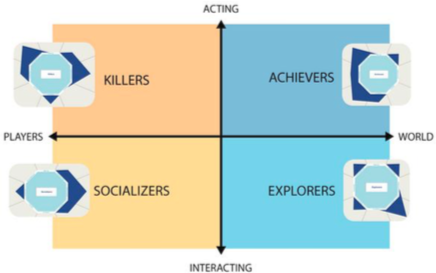
\includegraphics[keepaspectratio=true,scale=0.6]{figuras/perfiljogadores.png}
	\caption{Perfil de jogadores}
	Fonte: \cite{chou2017actionable}
	\label{perfiljogadores}
\end{figure}

Na figura \ref{nivel3}, são apresentados os \textit{core drives} mais utilizados em cada uma das quatro fases da jornada dos jogadores levando em
consideração os quatro tipos de perfis identificados por \citeonline{bartle1996hearts}.

\begin{figure}[h]
	\centering
	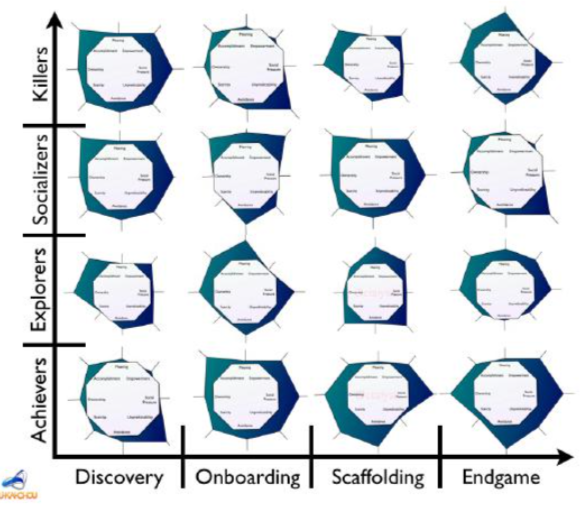
\includegraphics[keepaspectratio=true,scale=0.5]{figuras/nivel3.png}
	\caption{\textit{Core drives} mais utilizados de acordo com as fases e perfis de jogadores.}
	Fonte: \cite{chou2017actionable}
	\label{nivel3}
\end{figure}

% Os realizadores são fortemente motivados pelo Core Drive 2: Desenvolvimento e Realização, bem como pelo Core Drive 6: Escassez e Impaciência. Eles estão sempre tentando concluir seu próximo objetivo, o que os faz sentir-se realizados quando o fazem. É claro que, até certo ponto, eles também se preocupam em usar sua criatividade para superar desafios, além de acumular os resultados de seu sucesso (unidades principais 3 e 4).
% Os exploradores são motivados predominantemente pelo Core Drive 7: imprevisibilidade e curiosidade, que os leva a descobrir novos conteúdos que nunca viram antes. Também existem sementes do Core Drive 2, 3 e 6. Eles usam continuamente sua criatividade para encontrar novas maneiras de testar todos os limites que os limitam e, quando obtêm sucesso, são cumpridos por um sentimento de realização.
% Os socializadores são motivados principalmente pelo Core Drive 5: influência social e relacionamento. Eles gostam de se misturar com os outros e se relacionar. Em menor escala, eles também são levados a pensar em maneiras inteligentes de envolver mais os outros (Core Drive 3), desfrutam de informações novas ou imprevisíveis ou até mesmo fofocas (Core Drive 7) e às vezes se tornam territoriais com seus amigos (Core Drive 4) )
% Por fim, os Killers são motivados principalmente por uma mistura de Core Drive 2: Desenvolvimento e Realização e Core Drive 5: Influência Social da Relação. Eles não apenas precisam se esforçar para atingir objetivos altos, mas precisam que outros reconheçam suas realizações e sua superioridade. Em um sentido menor, eles também são levados a encontrar a melhor maneira de derrotar a competição (Core Drive 3), evitar serem mortos ou vistos como fracos (Core Drive 8) e, finalmente, contar suas vitórias e vitórias ( Unidade de núcleo 4).


% Com o gráfico acima, podemos entender melhor o que motiva exclusivamente esses tipos de jogadores e podemos projetar técnicas de jogo apropriadas para eles. Posteriormente em sua jornada de Octalysis, você começará a investir uma quantidade significativa de esforços na definição de seus próprios tipos de jogadores e no design de sistemas que os atraem exclusivamente com a oclise nível 3. Infelizmente, não podemos cobrir isso no escopo deste livro.
% Então, o que acontece com os outros Drives Principais que não são abordados acima, como Significado Épico e Chamado e, até certo ponto, Perda e Evitação?
% O Core Drive 1: Significado e Chamadas Épicas pode ser utilizado por qualquer um dos Tipos de Jogadores: para atingir seus objetivos de atingir um objetivo mais alto, tornando-se mais respeitados por seus amigos, explorando novas áreas e derrotando jogadores mais fracos.
% É simplesmente o contexto para estar no ambiente de jogo em primeiro lugar. Mas como Richard Bartle estava criando um mundo virtual aberto, não parece haver nenhum senso real de missões superiores ao idealismo do mundo virtual. quando os usuários de um mundo virtual se unem para uma missão mais alta na qual acreditam. Mas isso é independente dos tipos de jogadores estudados aqui.
% No modelo de Andrzej Marczewski, existe um tipo de usuário único no local de trabalho chamado Filantropos, que são indivíduos que obtêm alegria e, portanto, brincam, ajudando os outros. Eles são motivados pelo Core Drive 1: Significado e vocação épicos, e as empresas devem incentivar o comportamento dos filantropos para garantir esforços mais colaborativos e um trabalho em equipe mais forte. Infelizmente, a maioria dos ambientes da empresa castiga os filantropos enquanto recompensa aqueles que buscam exclusivamente suas próprias recompensas extrínsecas. Esses jogadores no modelo de Andrzej Marczewski são altamente motivados pelo Core Drive 4: Propriedade e posse, onde o objetivo é maximizar seus bônus, recompensas, promoções e aumentos de salário.
% Em termos do Core Drive 8: Perda e Prevenção, sempre há ameaças por não ter sucesso em nenhum empreendimento. Especialmente, como mencionado anteriormente, quando Killers tenta evitar ser humilhado. No entanto, não existe um tipo de jogador real que se concentre em evitar coisas ruins. Como aprendemos, se você é motivado apenas pela Black Hat Drives, em primeiro lugar não vai querer estar em um mundo aberto e voluntariamente virtual. Geralmente, essa é uma história diferente para o local de trabalho.
% No final do dia, esses oito Drives Principais nos motivam até certo ponto, pois universalmente desejamos esses Drives Principais em diferentes medidas e em diferentes momentos. O Octalysis Framework nos permite entender se certas unidades principais são mais fortes com certas pessoas, para que possamos estar cientes e projetar essas diferenças adequadamente.


\section{Estudos semelhantes}
% Com o objetivo de apoiar o ensino e aprendizagem de programação, alguns autores investem no estudo e desenvolvimento
% de ferramentas que possam aumentar o interesse e engajamento de alunos na realização de determinadas atividade. Nesta
% seção, são apresentadas algumas tecnologias, segundo a literatura, que foram desenvolvidas com o objetivo de auxiliar
% alunos e professores no ensino e aprendizagem de programação.

% \section{Exemplo de Ferramenta gamificada existente}
Com o objetivo de apoiar o ensino e aprendizagem de programação, alguns autores investem no estudo e desenvolvimento
de ferramentas que possam aumentar o interesse e engajamento de alunos na realização de determinadas atividades. Nesta
seção, são apresentadas dois estudos, um desenvolvido por pesquisadores da Universidade Federal da Paraíba e outro por um aluno
da Universidade de Brasília. Ambos os trabalhos foram elaborados objetivando fornecer um meio de auxiliar o ensino e aprendizagem 
de programação nessas universidades.

É importante salientar que foram realizadas buscas por meio do portal de periódicos Capes, IEEE, google e outros meios e identificou-se
apenas as duas ferramentas apresentadas neste tópico com características semelhantes à proposta, sendo que apenas uma delas ("Ambiente de aprendizagem Gamificado para ensino de Algoritmos")
faz uso do \textit{framework Octalysis}. Isso não significa que não há outras ferramentas com as mesmas propostas, apenas indica que não foram identificadas neste trabalho.

\subsection{Ambiente de aprendizagem Gamificado para ensino de Algoritmos}

\citeonline{wilker}, em seu trabalho de conclusão de curso, apresentou uma proposta de gamificação baseada no \textit{framework Ocatalysis} nível 2, seu estudo baseou-se na
utilização e adaptação de três ferramentas de forma a propor atividades gamificadas que auxiliassem o aprendizagem de programação dos alunos.

Para a proposta foi criado um curso com duração de um mês que continha atividades que deveriam ser executas semanalmente pelo
jogador/alunos inscritos.

As ferramentas utilizadas e sua características são apresentadas logo em seguida.

\begin{itemize}
	\item Funifier: Ambiente voltado para a implementação de gamificação. Seu propósito está relacionado à gamificação de outros \textit{softwares}
		a partir de técnicas propostas por YuKai.
	\item Moodle: Consiste um uma plataforma de aprendizado criada com o objetivo de fornecer um ambiente seguro, robusto e integralizado.
		O moodle permite a criação de ambientes personalizados voltados para o aprendizado.
	\item Scratch: Linguagem de programação voltada para pessoas que nunca tiveram contato prévio com programação. A forma de programar lembra
		muito os tradicionais brinquedos de construção utilizando blocos.
\end{itemize}

Após realizar o levantamento das necessidades, \citeonline{wilker} dividiu seu modelo de gamificação em quatro fases que são propostas por \citeonline{chou2017actionable}.
As fases ou ciclo de vida de um projeto de gamificação são: descoberta, entrada, dia a dia e fim de jogo. Os detalhes destas fases podem ser encotradas na seção anterior.

A divisão das técnicas quanto as suas fases definidas pelo autor do estudo são apresentadas na figura \ref{fases}. 

\begin{figure}[h]
	\centering
	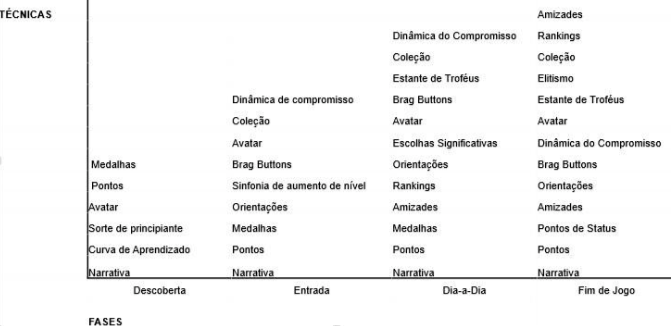
\includegraphics[keepaspectratio=true,scale=0.65]{figuras/fases.png}
	\caption{Distribuição das técnicas.}
	Fonte: \cite{wilker}
	\label{fases}
\end{figure}

\pagebreak

Com as técnicas definidas em cada fase, o passo seguinte foi realizar as adaptações necessárias e integrar as ferramentas de forma a criar
um fluxo de uso lúdico aos jogadores, na figura \ref{fluxo} pode-se observar o fluxo proposto aos estudantes.

\begin{figure}[h]
	\centering
	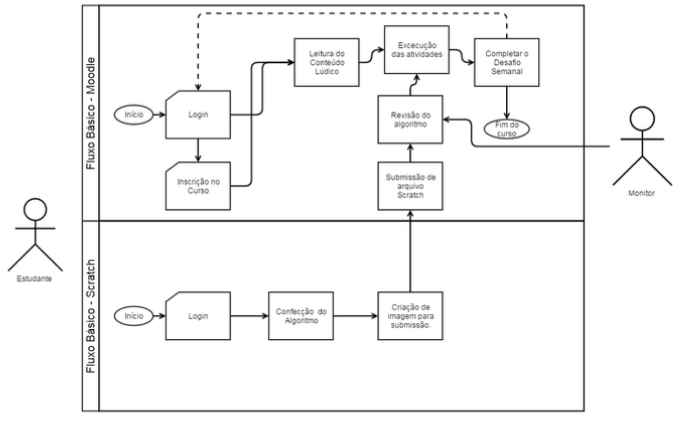
\includegraphics[keepaspectratio=true,scale=0.55]{figuras/fluxo.png}
	\caption{Fluxo de uso}
	Fonte: \cite{wilker}
	\label{fluxo}
\end{figure}

No modelo projetado, os jogadores são recompensados a medida que realizam as atividades propostas, duas das recompensas
implementadas são, por exemplo, o ganho de medalhas e pontos. Juntas, as ferramentas são capazes de oferecer aos alunos conteúdos 
, exercícios teóricos e práticos (Scratch) por meio de desafios que devem ser cumpridos semanalmente.

Embora o trabalho não tenha contado com feedbacks dos usuários, segundo \citeonline{wilker}, a proposta foi tida
como satisfatória, uma vez que os testes realizados apresentavam comportamentos esperados baseados na literatura, principalmente
Yukai, levantada pelo autor.

\subsection{Outros trabalhos semelhantes}
Nesta seção é apresentada uma ferramenta gamificada desenvolvida por pesquisadores da Universidade Federal da Paraíba a partir 
da utilização de técnicas alternativas ao \textit{framework Octalysis}. O estudo baseou-se no desenvolvimento de uma ferramenta para
auxiliar o aprendizado de programação dos alunos da própria universidade.

\subsubsection{O Desafio da Serpente}
Tendo em vista os problemas motivacionais e dificuldades enfrentadas por alunos de graduação no que se refere ao
aprendizado de programação do curso de computação da Universidade Federal
da Paraíba, \citeonline{raposo2016desafio} desenvolveram um jogo que foi disponibilizado na \textit{web} {\itshape} e apelidado
de "O Desafio da Serpente". O propósito da criação do jogo é estimular os alunos a praticarem diariamente seus conhecimentos
por meio de uma série de questões selecionadas e disponibilizadas pelo professor da disciplina.

O jogo envolve os alunos em uma batalha contra uma serpente que faz referência à linguagem de programação utilizada na
disciplina (\textit{python}{\itshape}). Para enfrentar e derrotar a serpente, os jogadores devem conquistar armas mediante o acúmulo
de pontos e resolução dos desafios propostos. 

Em seguida é apresentado um tabuleiro conceitual do jogo. No tabuleiro é possível
identificar por meio das diferentes cores as cinco fases propostas e as armas que podem ser conquistadas mediante a
resolução dos desafios. O uso do corpo da serpente como tabuleiro tem como objetivo apresentar o caminho sequencial que deve
ser seguido pelos jogadores em busca da vitória. Cada fase, representadas pelas cores na figura \ref{figura1}, correspondem a um conteúdo
que deve ser estudado pelos jogadores.

\begin{figure}[h]
	\centering
	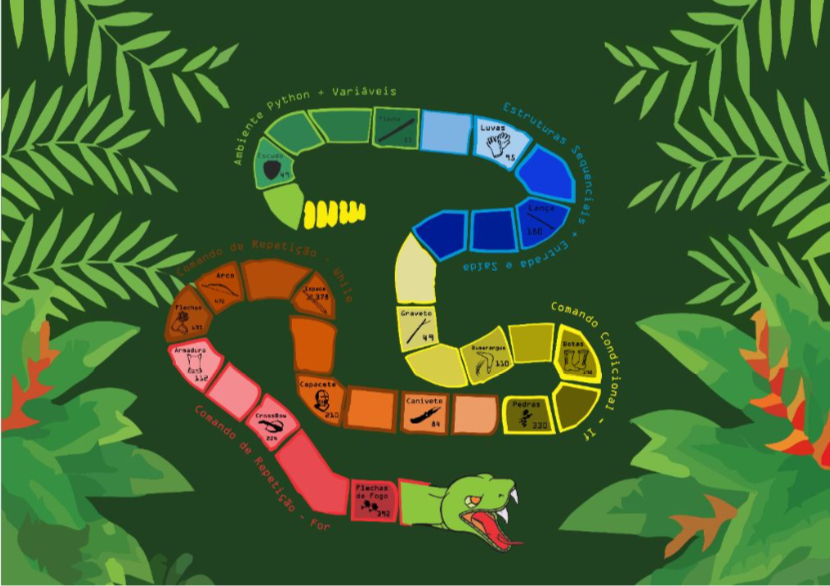
\includegraphics[keepaspectratio=true,scale=0.25]{figuras/desafioSerpente.png}
	\caption{Representação conceitual do jogo}
	Fonte: \cite{raposo2016desafio}
	\label{figura1}
\end{figure}

\pagebreak

Todos os dias da semana, de segunda a sexta feira, eram disponibilizados desafios que continham de duas a seis
questões dos mais variados níveis de complexidade, permitindo que os jogadores, ao concluírem os desafios propostos, 
conquistassem pontos e adquirissem armas. O objetivo era estimular os jogadores a estabelecerem uma rotina de estudos,
dedicando diariamente algum tempo para a resolução de exercícios voltados para a programação.

As questões foram classificadas em três níveis de complexidade (fácil, médio e difícil), na tabela a seguir, apresenta-se
as características de cada um destes níveis.

\begin{table}[h]
	\centering
	\resizebox{\textwidth}{!}{%
	\begin{tabular}{|l|l|l|l|}
	\hline
	\textbf{Complexidade} & \textbf{Tipo de Questão} & \textbf{Tempos estimado para resposta} & \textbf{Quantidade máxima de questões por dia} \\ \hline
	Fácil & \begin{tabular}[c]{@{}l@{}}V ou F\\ Teórica Objetiva\end{tabular} & 5 minutos & 8 \\ \hline
	Médio & \begin{tabular}[c]{@{}l@{}}Acompanhamento\\  (Teste de Mesa)\end{tabular} & 10 minutos & 4 \\ \hline
	Difícil & \begin{tabular}[c]{@{}l@{}}Elaboração de\\ Programas\end{tabular} & 20 minutos & 2 \\ \hline
	\end{tabular}%
	}
	\caption{Classificação das questões}
	Fonte: \cite{raposo2016desafio}
	% \small{Quadro 1 - Classificação das questões, \citeonline{raposo2016desafio}} 
\end{table}

Objetivando manter os jogadores motivados, cada fase possuia um sistema de \textit{ranking}{\itshape} independente
das fases anteriores, desta forma, mesmo que um jogador não tivesse obtido uma boa pontuação nas fases anteriores, ele
começaria a fase seguinte sem desvantagem em relação aos demais jogadores. 

A medida que os jogadores acumulavam pontos, os mesmos conquistavam novas armas para combater a serpente. Estas armas podiam
ser de defesa (escudos, armaduras e etc) ou de ataque (espada, lança e etc). O objetivo era fazer com que os jogadores conseguissem conquistar
o maior número possível de armas em cada fase. Cada armamento possuia uma quantidade mínima de pontos necessários para sua
aquisição e possuiam apenas funções simbólicas.

\begin{figure}[h]
	\centering
	
\includegraphics[keepaspectratio=true,scale=0.45]{figuras/armas.png}
	\caption{Exemplos de armas e pontuações}
	Fonte: \cite{raposo2016desafio}
	\label{figura2}
\end{figure}

\pagebreak

Além de permitir que os jogadores colecionassem pontos e armas, os primeiros jogadores tinham sua fotos expostas no
site do jogo, exaltando suas conquistas.

Para motivar os alunos a utilizarem a ferramenta e possibilitar a coleta de dados que permitissem analisar o 
impacto do uso da tecnologia gamificada no ensino de programação, foi acordado que, os alunos que obtivessem 
um aproveitamento de no mínimo 70\% em todas as fases do jogo, receberiam um ponto extra na primeira unidade 
da disciplina. Os alunos que obtivessem nota superior ou igual a 50\% em todas as fases do jogo, receberiam 
meio ponto extra na nota da primeira unidade da disciplina. Desta forma, a participação no jogo teria caráter 
voluntário e não estaria diretamente ligado às avaliações da disciplina. Recompensar os alunos com pontos extras
tinha como objetivo identificar até que ponto a motivação dos jogadores em solucionar os desafios seria ocasionado
pelo próprio jogo e não por pontos.

Considerando as quatro primeiras semanas de aula utilizando a ferramenta, os resultados foram bastante animadores.
Do total de 106 alunos que realmente frequentaram as aulas, apenas quatro não participaram de nenhum dos desafios 
propostos, o que indica que a aceitação da ferramenta pelos alunos foi de mais de 96\% . Além destes indicadores 
quantitativos, \citeonline{raposo2016desafio} relatou em sua pesquisa que a empolgação dos alunos na utilização da 
ferramenta era bastante perceptível. Muitos alunos se diziam bastante ansiosos para o desafio do dia e notou-se um 
grande aumento no número de discussões a respeito das questões durante as aulas.

\subsection{Engenharia de \textit{software}}

Como apresentado por \cite{tripp1994ieee}, a engenharia de software consiste na aplicação de uma abordagem sistemática, discplinada
e quantificável no desenvolvimento, na manutenção e operação de software, ou seja, é aplicação da engenharia ao
software.

No livro "Engenharia de Software: Uma abordagem tradicional", \citeonline{pressman} diz que a engenharia de software é
uma tecnologia em camadas que deve ter como foco o comprometimento com a qualidade. O autor apresenta quatro camadas que
são, na visão dele, as principais camadas presentes na engenharia de software. 

\pagebreak

\begin{figure}[h]
	\centering
	
\includegraphics[keepaspectratio=true,scale=0.45]{figuras/camada.png}
	\caption{Camadas da engenharia de software}
	Fonte: \cite{pressman}
	\label{figura123}
\end{figure}

O processo é a fonte que mantém as camadas de tecnologia coesas e possibilita que se desenvolva o software de 
forma racional e dentro dos prazos estabelecidos. O processo de software permite o controle e gerencimento de
projetos onde  a qualidade é garantida e mudanças são geridas de forma apropriada.

A camada denominada métodos envolve uma ampla gama de tarefas, que incluem: análise de requisitos, modelagem,
comunicação, construção de programa, testes e suporte. Os métodos da engenharia de software baseiam-se em um 
conjunto de princípios básicos que gerenciam cada área da tecnologia e inclui diversas atividades, como as
apresentadas neste parágrafo.

A camada superior, denominada ferramentas, referem-se às tecnologias de \textit{software} que fornecem suporte
automatizado ou semiautomatizado para o processo e para os métodos.

\subsubsection{Metodologia cascata}

De acordo com \citeonline{semedo2012ganhos}, metodologia pode ser definida como um conjunto de procedimentos, técnicas, documentação e ferramentas que 
auxiliam os responsáveis ou interessados no desenvolvimento e implementação de um sistema de informação. Na maioria das vezes, o sucesso
de um projeto de software depende de vários fatores que vão desde o planejamento à escolha mais adequada de uma metodologia.

O modelo cascata, também conhecido como modelo tradicional, é uma das metodologias mais antigas e conhecidas. A utilização desta 
metodologia consiste em seguir o desenvolvimento do projeto de forma sequencial, onde só se deve passar para os níveis seguintes após
a conclusão do nível anterior. Esta metodologia envolve duas grandes fases: levantamento de requisitos/necessidades e design. \cite{semedo2012ganhos}

Muitos autores desencorajam a utilização da metodologia cascata no desenvolvimento de grandes sistemas, como é o caso do pesquisador
\apudonline{gilb1988principles}{semedo2012ganhos}  e \apudonline{brooks}{semedo2012ganhos}. Este tipo de metodologia deve ser usada apenas em situações onde os requisitos do software são estáveis e requisitos
que possam vir a surgir no futuro sejam previsíveis. \cite{semedo2012ganhos}


No modelo cascata apresentado por \citeonline{pressman} no livro "Engenharia de Software: Uma abordagem profissional", o autor
apresenta cinco fases sequenciais que devem ser satisfeitas no desenvolvimento de um sistema obedecendo esta metodologia(cascata). 
Cada uma das cinco fases podem ser vistas na figura \ref{cascata} apresentada logo em seguida.

\begin{figure}[h]
	\centering
	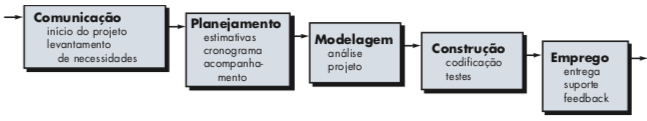
\includegraphics[keepaspectratio=true,scale=0.6]{figuras/cascata.png}
	\caption{Modelo cascata}
	Fonte: \cite{pressman}
	\label{cascata}
\end{figure}


\subsubsection{Engenharia de requisitos}

A engenharia de requisitos é uma importante área dentro da engenharia de \textit{software}. Ela tem início na fase mais
inicial dos projetos de \textit{software} , a comunicação e se perpetua até a fase de modelagem e deve ser adaptada às 
necessidades do processo, projeto, produto e pessoas que estão envolvidas no trabalho \cite{pressman}.

A engenharia de requisitos fornece apoio e técnicas apropriadas para entender aquilo que o cliente quer, 
analisando suas necessidades, negociando soluções razoáveis para o tipo de problema, avaliando a viabilidade
entre outras características que permitem o desenvolvimento de soluções que atendam às demandas dos usuários \cite{pressman}.

\subsubsubsection{Priorização de requisitos: \textit{Moscow}}

Como apresentado por \citeonline{pressman}, há diversas formas de se elicitar requisitos, seja por meio de reuniões
com clientes ou por meio de questionários, o importante é entender quais são as necessidades e urgências dos clientes
e buscar atendê-las da melhor forma possível, levando em considaração metodologias e técnicas da engenharia de software.

A técnica de priorização \textit{Moscow}, consiste na utilização de um quadro dividido em quatro colunas que servem como ``classificadores''
de prioridade \cite{moscow}.

Logo em seguida são apresentados resumidamente cada um das quatro possíveis classificações abordadas pela técnica.

\begin{itemize}
	\item  \textit{Must Have}: nesta coluna vão todos os requisitos que são críticos ou obrigatórios para a construção do sistema. Se um dos ítens
não é concluído, o projeto não é considerado bem sucedido;
	\item  \textit{Should Have}: ítens com classificação \textit{should} são importantes mas não são necessários para entrega em um primeiro 
momento. São ítens tão importantes quanto os classificados como \textit{must}, mas em geral não são críticos ou pode-se esperar um pouco para ser
trabalhado;
	\item \textit{Could Have}: ítens com esta classificação são desejáveis, mas não são necessários. Geralmente podem ser atendidos quando 
houver tempo e recursos disponíveis para sua realização.
	\item \textit{Would Have}: ítens com esta classificação são os menos críticos ou não são adequados para serem realizados durante algum
período de tempo.
\end{itemize}

Segundo \citeonline{moscow}, algumas vantagens de se utilizar a técnica \textit{moscow} são: facilidade de compreensão, facilidade de trabalho, linguagem simples
entre outras. É importante salientar que se trata de uma técnica subjetiva quando se refere à classificação dos ítens e por este motivo, demanda de um 
bom entendimento do problema que se tem a intenção de resolver, de forma a melhor identificar quais ítens são de fato prioridades em relação à outros ítens.

\begin{figure}[h]
	\centering
	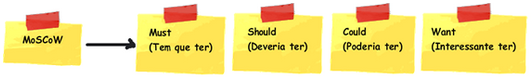
\includegraphics[keepaspectratio=true,scale=0.75]{figuras/moscow.png}
	\caption{Exemplificação da classificação de ítens quanto à sua prioridade}
	Fonte: \cite{moscow}
	\label{moscow}
\end{figure}

Na figura \ref{moscow} é apresentado uma esquematização simplificada quanto à forma correta de utilização do \textit{moscow} como 
técnica de priorização de requisitos. É possível notar a redução gradativa da prioridade dos ítens quanto a sua necessidade
e urgência de desenvolvimento. 


\chapter{Metodologia}
Neste capítulo são apresentados com detalhes o passo a passo a ser realizado para a contrução de uma ferramenta \textit{web}
de apoio ao ensino e aprendizagem de programação gamificada, bem como os passos dados para levantar os requisitos necessários
para sua construção.

Como apresentado no referencial teórico deste trabalho, o \textit{framework octalysis} é dividido em vários níveis. Neste
trabalho, será abordado o nível 1. 

\section{Fase 1: Coleta de informações }

\subsection{Elicitação de requisitos}
Com o objetivo de levantar requisitos para a construção da ferramenta de apoio ao ensino e aprendizagem de 
programação, foi elaborado um questionário para coletar informações a respeito da disciplina introdutória de programação 
do campus Gama (FGA) da Universidade de Brasília na visão dos alunos que cursaram ou estão cursando a disciplina. Também 
foram incluidas  questões relacionadas aos \textit{games} com o objetivo de identificar alguns mecanismos característicos
de jogos que pudessem ser incluidos na construção da ferramenta levando em consideração o  \textit{framework octalysis}
apresentado no capítulo 2 deste trabalho.

Ao se concluir a pesquisa baseada no questionário, iniciou-se a pesquisa por plataformas gamificadas semelhantes, buscando
identificar os mecanismos mais utilizados nestas ferramentas (sistema de \textit{ranking}, disputas e etc), usabilidade (layouts, responsividade e etc) entre outras.

Nas subseções a seguir, são apresentadas em detalhes a elaboração e resultados obtidos a partir das pesquisas realizadas.

\subsubsection{Questionário}
Para realizar a coleta de informações que permitissem a identificação dos requisitos e \textit{core drives}, foi elaborado um questionário 
contendo 33 perguntas referentes à disciplina Algoritmos de Programação de Computadores, algumas outra perguntas
relacionadas a jogos na perspectiva do participante do questionário. Algumas questões do questionário foram baseadas no \textit{survey}
da \textit{University of Waterloo}, que possui perguntas que ajudam na identifação de preferências de jogadores.
Em seguida, o questionário foi publicado em um grupo na rede social \textit{facebook} que contém
vários estudantes dos cursos de engenharias da Universidade de Brasília (UnB), campus Gama (FGA). O mesmo questionário
também foi disponibilizado em um grupo no \textit{telegram} da engenharia de software criado pelos próprios estudantes do
curso. 

Disponibilizar o questionário no grupo do \textit{facebook} em que se encontram alunos de cada uma das cinco engenharias ofertadas no campus (FGA)
teve como objetivo reunir o maior número possível de informações sobre a perspectiva de diferentes perfis de alunos que cursam, cursaram ou vão
cursar a disciplina introdutória de programação.

O questionário contou com a participação 58 alunos. A quantidade e percentual de participantes por curso podem ser apreciadas na tabela \ref{participantes} e
na figura \ref{graficocurso}.

\begin{figure}[h]
	\centering
	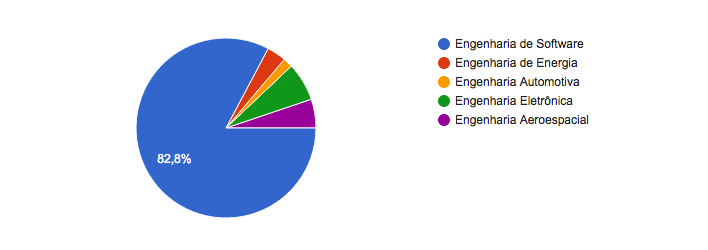
\includegraphics[keepaspectratio=true,scale=0.75]{figuras/graficocurso.png}
	\caption{Gráfico resultante da pesquisa por curso.}
	Fonte: {Autor}
	\label{graficocurso}
\end{figure}


\begin{table}[h]
	\centering
	\resizebox{.8\textwidth}{!}{%
	\begin{tabular}{|l|l|l|l|}
	\hline
	\textbf{Curso} & \textbf{Quantidade} & \textbf{Percentual} \\ \hline
		Engenharia de Software & 48 alunos & 82,8\% \\ \hline
		Engenharia Aeroespacial & 03 alunos & 5,2\% \\ \hline
		Engenharia Eletrônica & 04 alunos & 6,9\% \\ \hline
		Engenharia de Energia & 02 alunos & 3,4\% \\ \hline
		Engenharia Automotiva & 01 aluno & 1,7\% \\ \hline
	\end{tabular}%
	}
	\caption{Participação no questionário}
	\label{participantes}
	Fonte: {Autor}
	% \small{Quadro 2 - Requisitos funcionais} 
\end{table}

\subsubsubsection{Escolha da linguagem de programação como foco de ensino}
Embora a construção da ferramenta será feita de forma a permitir a inclusão de várias linguagens de programação, a linguagem C será
utilizada como foco deste estudo. A decisão foi tomada com base no \textit{survey} realizado que continha uma pergunta voltada diretamente
para identificar as linguagens mais utilizadas na disciplina de "Algoritmos e Programação de Computadores". Os resultados da pesquisa podem
ser apreciados na figura \ref{linguagemc}.

\begin{figure}[h]
	\centering
	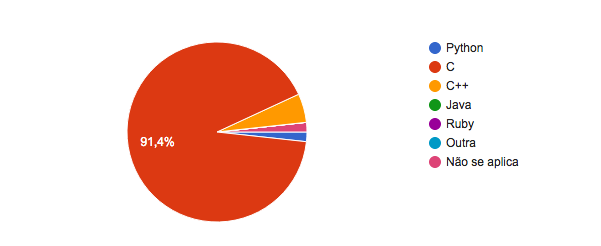
\includegraphics[keepaspectratio=true,scale=0.75]{figuras/linguagemc.png}
	\caption{Linguagens de programação utilizadas em APC.}
	Fonte: {Autor}
	\label{linguagemc}
\end{figure}

\subsubsubsection{Características de \textit{design}}
Com o questionário, buscava-se também identificar os \textit{games} mais jogados pelos estudantes. Desta forma, o questionário continha uma
pergunta dissertativa que permitia aos participantes informarem um ou mais jogos que o mesmo estava engajado. O objetivo era utilizar 
a plataforma/site do jogo como fonte de extração de características de \textit{design} que poderiam vir a ser incorporadas na ferramenta a ser
desenvolvida.

Na figura \ref{gamejogados}, é possível notar a distribuição das respostas quanto a preferência dos jogos.

\pagebreak

\begin{figure}[h]
	\centering
	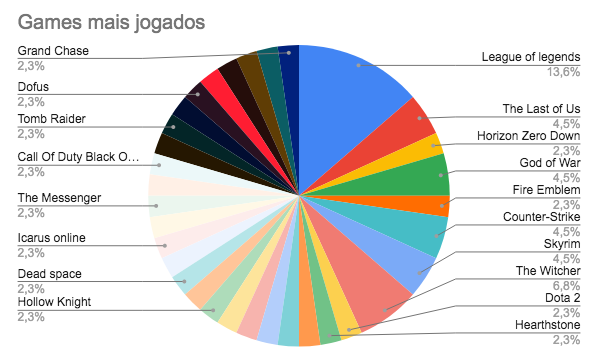
\includegraphics[keepaspectratio=true,scale=0.75]{figuras/gamejogados.png}
	\caption{Gráfico resultante da pesquisa por preferência de jogos.}
	Fonte: {Autor}
	\label{gamejogados}
\end{figure}

Tendo como base os resultados da pesquisa, o \textit{website} do jogo \textit{"League of Legends"} será utilizado como base para a extração de algumas
características visuais a serem implementadas.

As perguntas realizadas podem ser encontradas no apêndice \ref{apendicea} deste trabalho.

% tabela com as perguntas aqui e percentual de respostas em uma das coluna
\subsubsection{Ferramentas Semelhantes}
Algumas ferramentas disponibilizadas na \textit{web} já apresentam características de jogos e , por conta disso,
atraem um grande público que utilizam destes recursos para aprimorar seus conhecimentos em programação, como é
o caso da plataforma \textit{Uri Online Judge} que é utilizada por cerca de 101.238 usuários atualmente e está disponível em três
idiomas, incluindo o português.
Nesta seção são apresentadas algumas das tecnologias gamificadas voltadas para o ensino e prática de programação
gamificadas. Algumas características de \textit{games} identificadas nestas ferramentas serão utilizadas como fonte
para o desenvolvimento da ferramenta proposta ao se notar sua grande utilização e aceitação após a comparação com as 
informações coletadas com o questionário.

\subsubsubsection{\textit{URI Online Judge}}
O URI Online Judge é uma ferramenta online disponível em três idiomas que permite que interessados em aprender ou
aprimorar seus conhecimentos em programação possam faze-lo de forma gamificada e intuitiva. A ferramenta possui três
formas de rankeamento que são: individual, por universidade ou por país. Até a data de publicação deste trabalho, o Brasil
lidera o \textit{ranking} de exercícios resolvidos e quantidade de usuários com 37.23.579 de exercícios resolvidos e cerca
de 101.238 usuários. \cite{URI} 

A ferramenta permite que seus usuários criem times e participem de torneios de duração que variam de trinta minutos até no 
máximo cinco dias, onde os jogadores batalham uns contra os outros na resolução de problemas relativos à programação.

O URI possui nove categorias de problemas que vão do nível mais básico (iniciante) até os mais complexos envolvendo grafos,
geometria computacional, linguagem sql entre outros.

Além da grande diversidade de categorias de problemas, a ferramenta permite que o usuário escolha a linguagem que deseja
praticar suas habilidades e conhecimentos em programação. No total são dezoito linguagens de programação que o jogador pode 
escolher.

\subsubsubsection{\textit{Data camp}}
O \textit{Data Camp} é uma plataforma de ensino de programação voltada principalmente para \textit{data science}.
A plataforma possui tutoriais em vídeo e desafios que podem ser solucionados utilizando uma das linguagens de programação
que a plataforma oferece suporte. \cite{datacamp}

Possui cerca de 4.770.000 usuários que se empenham em solucionar os mais diversos problemas propostos pela plataforma. Os usuários
podem  utilizar a própria plataforma para desenvolver e submeter seus códigos que passam por analisadores que corrigem a solução submetida.

A ferramenta ainda conta com a opção de criação de grupos onde os participantes do mesmo são apresentados em um \textit{ranking} 
de acordo com a pontuação que vão conquistando a medida que concluem os desafios, capítulos e cursos propostos para todo o grupo.

\subsubsection{\textit{Computer Science Education Week}}
O CSEW é uma ferramenta \textit{online} focado no ensino de programação por meio de gamificação. A plataforma possui
diversos desafios que variam da criação de programas simples até o desenvolvimento de jogos. O foco é ensinar lógica de programação 
por meio de blocos lógicos que ao serem ``montados'' em uma determinada sequência lógica, produz resultados visuais, permitindo uma melhor
compreensão dos jogadores sobre a lógica envolvida.

Até o momento de publicação deste trabalho, a plataforma contava com cerca de 835.122.270 submissões de soluções.

\subsection{Priorização de requisitos}
Após concluir a coleta de informações, foi elaborado a tabela que é apresentada logo em seguida contendo os requisitos
identificados.

\begin{table}[h]
	\centering
	\resizebox{.8\textwidth}{!}{%
	\begin{tabular}{|l|l|l|l|}
	\hline
	\textbf{Identificador} & \textbf{Requisito}\\ \hline
	RF 01 & CRUD de jogadores \\ \hline
	RF 02 & Ativar/desativar perfil de jogadores \\ \hline
	RF 03 & Rankeamento de jogadores\\ \hline
	RF 04 & CRUD de disciplinas \\ \hline
	RF 05 & CRUD de turmas \\ \hline
	RF 06 & CRUD de conteúdos para estudo\\ \hline
	RF 07 & CRUD de desafios \\ \hline
	RF 08 & Sistema de recompensas (pontuação) \\ \hline
	RF 09 & Dashboard pessoal de desempenho (jogadores)  \\ \hline
	RF 10 & CRUD de professores de disciplinas\\ \hline
	RF 11 & Painel de acompanhamento de desempenho dos alunos (professores) \\ \hline
	RF 12 & Narrativa temática \\ \hline
	RF 13 & Personagens e guerreiros da narrativa \\ \hline
	RF 14 & Lógica de progressão de jogadores (\textit{levels})\\ \hline
	RF 15 & CRUD de linguagens de programação \\ \hline
	RF 16 & Desafios entre jogadores (individual) \\ \hline
	RF 17 & CRUD de questões \\ \hline
	RF 18 & Desafios entre times/grupos \\ \hline
	RF 19 & Torneios/campeonatos entre turmas \\ \hline
	\end{tabular}%
	}
	\caption{Requisitos Funcionais}
	Fonte: {Autor}
	% \small{Quadro 2 - Requisitos funcionais} 
\end{table}

Com base na tabela apresentada anteriormente, utilizou-se a técnica de priorização \textit{moscow} para realizar
a priorização dos requisitos. As características desta técnica podem ser apreciadas no referencial teórico deste trabalho.

Na tabela \ref{prioridade}, são apresentados os requisitos priorizados a partir desta técnica (\textit{moscow}.

\begin{table}[h]
	\centering
	\resizebox{\textwidth}{!}{%
	\begin{tabular}{|p{6cm}|p{6cm}|p{6cm}|p{6cm}|}
	\hline
	\textbf{\textit{Must}} & \textbf{\textit{Should}} & \textbf{\textit{Could}} & \textbf{\textit{Would/Wont}} \\ \hline
		RF 01 & RF 09 & RF 02 & RF 18  \\ \hline
		RF 03 & RF 10 & RF 11 & RF 19  \\ \hline
		RF 04 & RF 15 & - & -  \\ \hline
		RF 05 & RF 16 & - & -  \\ \hline
		RF 06 & - & - & -  \\ \hline
		RF 07 & - & - & -  \\ \hline
		RF 08 & - & - & -  \\ \hline
		RF 10 & - & - & -  \\ \hline
		RF 12 & - & - & -  \\ \hline
		RF 13 & - & - & -  \\ \hline
		RF 14 & - & - & -  \\ \hline
		RF 17 & - & - & -  \\ \hline

	\end{tabular}%
	}
	\caption{Requisitos priorizados utilizando \textit{moscow}}
	\label{prioridade}
	Fonte: autor
	% \small{Quadro 1 - Classificação das questões, \citeonline{raposo2016desafio}} 
\end{table}

\subsection{Escolha do \textit{framework Octalysis}}
Com base na quantidade de trabalhos em gamificação que utilizaram o \textit{framework Octalysis} como suporte para o desenvolvimento de 
uma proposta de gamificação nas mais diversas áreas, existência de uma grande quantidade de material disponível para o estudo, 
existência de comunidades ativas voltadas para a resolução de dúvidas e dificuldades de usuários iniciantes e existência de ferramentas 
que possibilitam a construção de um modelo próprio de gamificação, decidiu-se utilizar o \textit{Octalysis} como modelo de gamificação a
ser seguido.

\subsection{Implementação de \textit{core drives}}

% Por meio da análise da figura \ref{perfiljogadores} e da tabela \ref{perfil}, é possível notar os principais \textit{core drives} 
% presentes em cada um dos perfis de jogadores. Por meio destes dois artefatos e utilizando-se dos resultados do questionário , é possível 
% identificar os perfis predominantes dentro do grupo para o qual a proposta de desenvolvimento da ferramenta está sendo direcionada 
% (alunos da FGA).

Para a realizar a escolha dos \textit{core drives} principais a serem implementados, utilizou-se os dados coletados por meio do questionário
\ref{apendicea}. Como apresentado no referencial teórico deste trabalho, existem oito núcleos quando se leva em consideração o \textit{framework Octalysis},
tendo isso em mente, a seção dois do questionário foi elaborada com três afirmações para cada \textit{core}, totalizando 24 afirmações, que deveriam ser julgadas
pelos participantes de acordo com a relevância/importância que este dá ao item. O intervalo de relevância foi elaborado com uma escala de variação de 0 a 10 e, quanto mais alto
fosse o valor selecionado, maior seria a importância dada ao item pelo participante.

Atribuiu-se pesos para os valores do intervalo de relevância, quanto maior o valor da escala, maior é o pesoa aplicado sobre ele. A distribuição dos pesos
é apresentado na tabela \ref{distribuicao}.

\begin{table}[h]
	\centering
	\resizebox{\textwidth}{!}{%
	\begin{tabular}{|p{6cm}|p{6cm}|}
	\hline
	\textbf{Valor na escala} & \textbf{Peso} \\ \hline
		0  &  1 \\ \hline
		1  &  2\\ \hline
		2  &  3 \\ \hline
		3  &  4 \\ \hline
		4  &  5 \\ \hline
		5  &  6 \\ \hline
		6  &  7 \\ \hline
		7  &  8 \\ \hline
		8  &  9 \\ \hline
		9  &  10 \\ \hline
		10 &  11\\ \hline
	\end{tabular}%
	}
	\caption{Distribuição dos pesos na escala}
	\label{distribuicao}
	Fonte: Autor
	% \small{Quadro 1 - Classificação das questões, \citeonline{raposo2016desafio}} 
\end{table}

O cálculo que permite identificar os \textit{core} com maior relevância de acordo com os participantes do questionário é apresentado 
na equação \ref{calculo}.

\begin{equation}
	\label{calculo}
	\scriptstyle CDX = \frac{((qtdVotosIxQx * pesoEscala) + (qtdVotosIxQx * pesoEscala) + (qtdVotosIxQx * pesoEscala)) }{3}
\end{equation}

Sendo que $CDX$ representa o \textit{Core drive} de número x, $qtdVotosIxQx$ é a quantidade de votos em um determinado 
item x de uma determinada questão x e $pesoEscala$ é o peso atribuído a cada item/valor (tabela \ref{distribuicao}).

Para tornar os cálculos mais eficientes e diminuir as chances de ocorrência de erros, foi elaborado um script que automatizou
os cálculos. Os resultados são apresentados na tabela \ref{calculos}. O script utilizado pode ser apreciado no apêndice \ref{script}.
% \pagebreak

\begin{table}[h]
	\centering
	\resizebox{\textwidth}{!}{%
	\begin{tabular}{|p{6cm}|p{6cm}|}
	\hline
	\textbf{\textit{Core drive}} & \textbf{Valor} \\ \hline
		Significado épico e chamado &  517,67  \\ \hline
		Desenvolvimento e conquista  &  538,67 \\ \hline
		Empoderamento e feedback  &  519,67 \\ \hline
		Propriedade e posse  &   509,33\\ \hline
		Influência e relacionamento social  &  509 \\ \hline
		Escassez e impaciência  &  437,33 \\ \hline
		Imprevisibilidade e curiosidade  &  394,33 \\ \hline
		Prevenção e perda  &  419,67 \\ \hline
	\end{tabular}%
	}
	\caption{Resultados dos cálculos de relevância.}
	\label{calculos}
	Fonte: Autor
	% \small{Quadro 1 - Classificação das questões, \citeonline{raposo2016desafio}} 
\end{table}

Tendo como base os valores obtidos, os quatro principais \textit{core drives} a serem utilizados na ferramenta são: "Desenvolvimento e conquista" (DC 2), "Empoderamento
e \textit{feedback}" (DC 3), "Significado épico e chamado" (DC 1) e "Prevenção e perda" (DC 8).

As técnicas a serem utilizadas são apresentadas na tabela \ref{tecnicas}.


\begin{table}[h]
	\centering
	\resizebox{\textwidth}{!}{%
	\begin{tabular}{|p{6cm}|p{6cm}|}
	\hline
	\textbf{\textit{Core drive}} & \textbf{Técnicas} \\ \hline
		Desenvolvimento e conquista &  Pontos, \textit{ranking}, lista de desafios, prêmios e barra de progresso. \\ \hline
		Empoderamento e \textit{feedback} &  Desbloqueio de marcos e \textit{feedback}\\ \hline
		Significado épico e chamado & Narrativa, sorte de iniciante e elitismo \\ \hline
		Prevenção e perda & Perda de progresso e perda de pontos\\ \hline
	\end{tabular}%
	}
	\caption{Técnicas a serem utilizadas.}
	\label{tecnicas}
	Fonte: Autor
	% \small{Quadro 1 - Classificação das questões, \citeonline{raposo2016desafio}} 
\end{table}

É importante ressaltar que pode haver a inclusão ou diminuição na quantidade de técnicas e \textit{core drives} a serem implementados.

As respostas obtidas por meio do questionário podem ser apreciadas no apêndice \ref{respostas}.

% COLOCAR AQUI O GRAICO OCTALYSIS DO MEU MODELO RESULTANTE.

\subsection{Plano pedagógico}

Nesta subseção são apresentados os conteúdos que se espera abordar no ensino de programação por meio da ferramenta gamificada. É importante  
ressaltar que devido a grande quantidade de conteúdos e devido a dificuldade da criação e seleção de conteúdos relevantes aos usuários, pode 
ser que ocorra em um primeiro momento apenas a inclusão de alguns assuntos. 

A seleção e ordenação dos conteúdos foram realizadas com base nas informações curriculares apresentadas pela plataforma matrícula web em uma 
busca pelas disciplinas “computação básica” e “algoritmos e programação de computadores”. As informações podem ser apreciadas diretamente na 
plataforma ou por meio do anexo \ref{planocb} e anexo \ref{planoapc}. Alguns conteúdos não foram incluídos por não fazerem parte da nova grade curricular e escopo da 
disciplina “algoritmos e programação de computadores”.

A ordem de apresentação dos conteúdos aos usuários pela ferramenta é apresentado na tabela \ref{prioridade}.

\begin{table}[h]
	\centering
	\resizebox{\textwidth}{!}{%
	\begin{tabular}{|p{4cm}|p{8cm}|}
	\hline
	\textbf{Prioridade/ordem} & \textbf{Assunto} \\ \hline
		1º & Algoritmos  \\ \hline
		2º & Linguagem de programação \\ \hline
		3º & Tipos de dados \\ \hline
		4º & Entrada e saída de dados \\ \hline
		5º & Operações primitivas  \\ \hline
		6º & Variáveis e expressões  \\ \hline
		7º & Estruturas de decisão  \\ \hline
		8º & Laços de repetição \\ \hline
		9º & Vetores   \\ \hline
		10º & Matrizes  \\ \hline
		11º & Funções e Procedimentos  \\ \hline
		12º & Arquivos: Armazenamento e manipulação \\ \hline
	\end{tabular}%
	}
	\caption{Prioridade de conteúdos.}
	\label{prioridade}
	Fonte: autor
\end{table}


\section{Fase 2: Desenvolvimento da ferramenta}

\subsection{Metodologia utilizada}

No desenvolvimento da ferramenta, escolheu-se a metodologia cascata devido a natureza de desenvolvimento deste trabalho ser compatível com as 
catacterísticas propostas pela metodologia. O desenvolvimento da ferramenta parte da definição dos requisitos que deverão
ser atendidos, planejamento, desenvolvimento, testes e entrega final.

As características desta metodologia podem ser apreciadas em detalhes no referencial teórico deste trabalho.

\begin{figure}[h]
	\centering
	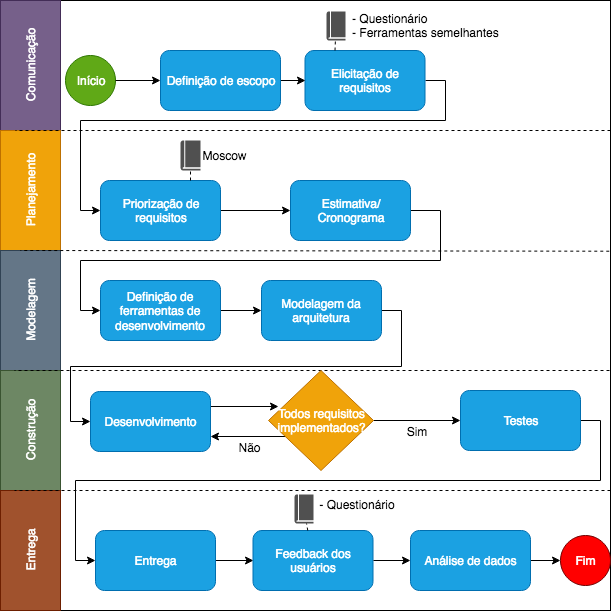
\includegraphics[keepaspectratio=true,scale=0.6]{figuras/modeloprocesso.png}
	\caption{Modelo de processos com principais atividades}
	Fonte: {Autor}
	\label{modeloprocesso}
\end{figure}	

No modelo apresentado na figura \ref{modeloprocesso}, é possível identificar em cada fase as principais atividades, iniciando pela definição
do escopo do projeto, elicitação de requisitos por meio da aplicação de um questionário e extração de algumas características
de \textit{design} de outras ferramentas e jogos, priorização dos requisitos por meio da ferramenta \textit{moscow},
 estimativa de desenvolvimento (disponível no tópico de cronogramas), definição das tecnologias de desenvolvimento a serem
 utilizadas, modelagem arquitetural da ferramenta a ser construída, desenvolvimento da ferramenta utilizando ferramentas e
 seguindo metodologia definida, testes do sistema de \textit{software}, disponibilização da versão a ser utilizada como foco 
de análise, coleta de \textit{feedback} por meio da aplicação de questionário e análise dos dados.  


\subsection{Tecnologias}

No desenvolvimento da ferramenta, escolheu-se as tecnologias com base nas seguintes características: afinidade
com as tecnologias de desenvolvimento, recursos disponibilizados pela tecnologia, qualidade e disponibilidade
de documentações e comunidades da tecnologia.

A seguir, são apresentadas tecnologias a serem utilizadas no desenvolvimento da ferramenta e suas características.

\begin{itemize}
	\item Java: Linguagem de programação orientada a objetos desenvolvida na década de 90.Diferente das linguagens de programação
		modernas que são compiladas para código nativo, a linguagem java é compilada para um \textit{bytecode} que é interpretado por uma máquina
		virtual (\textit{java virtual machine}). Por conta disso, a linguagem torna-se altamente portável, isto é, independente de plataforma \cite{java}.
	\item Vue.js: \textit{Framework} javaScript voltado para o desenvolvimento de interfaces de usuário \cite{vue}.
	\item MySql: Sistema de gerenciamento de banco de dados que utiliza linguagem sql como interface. Voltado para o armazenamento e manutenção 
		de registros de um banco de dados \cite{mysql}.
	\item Maven: Ferramenta de automação de compilação muito utilizada em projetos que envolvem a linguagem java. O maven
		utiliza um arquivo \textit{xml} (POM) para descrever o projeto de software sendo implementado, suas dependências, componentes
		externos, \textit{plugins} necessários, diretórios e ordem de compilação \cite{maven}.
	\item Jersey: \textit{Framework} que facilita o desenvolvimento de APIs (Application Programming Interface) RESTful \cite{jersey}.
	\item Axios: É um cliente HTTP que permite consumir e exibir dados de uma API (Application Programming Interface) de forma facilitada e ágil \cite{axios}.
	\item JDBC: \textit{Driver} que possui um conjunto de classes e interfaces java que permitem o envio/comunicação com qualquer
		banco de dados relacional. Permitindo interligar a aplicação com um banco de dados \cite{jdbc}.
	\item Html: Linguagem de marcação bastante utilizada na construção de páginas web. Que podem ser interpretados por 
		qualquer navegador \cite{html}.
	\item CSS: Mecanismo que permite adicionar cores, fontes, espaçamentos e efeitos em um documento \textit{web} (html). \cite{css}
	\item Bootstrap:\textit{Framework web} voltado para o desenvolvimento de interfaces para aplicações e sites usando HTML, CSS e JavaScript, melhorando
		a experiência do usuário, tornando um site amigável e responsível \cite{bootstrap}.
	\item Json: \textit{JavaScript Object Notation} é uma formatação de troca de dados. Possui formato textual e é completamente independente de linguagem. É
		consituido por conjuntos de chave e seu respectivo valor \cite{json}.
	\item Tomcat: Consiste em um servidor de aplicações java que permite que o mesmo funcione na \textit{web} \cite{tomcat}.

\end{itemize}

\subsection{Arquitetura}

No desenvolvimento da ferramenta, tem-se como modelo arquitetural a ser utilizado o "n camadas". Esse tipo
de arquitetura consiste na separação de responsabilidades específicas para cada uma das camadas presentes 
na construção do sistema \cite{MSF}. A letra ``n'' representa a quantidade de camadas em que a construção do sistema 
está dividida, para esta proposta de solução, o desenvolvimento do sistema será dividido em 4 camadas que são: apresentação, serviço, modelo
e armazenamento.

O modelo simplificado apresentado na figura \ref{arquitetura} demonstra como ocorre o fluxo de comunicação entre as principais tecnologias
usadas no desenvolvimento.

\begin{figure}[h]
	\centering
	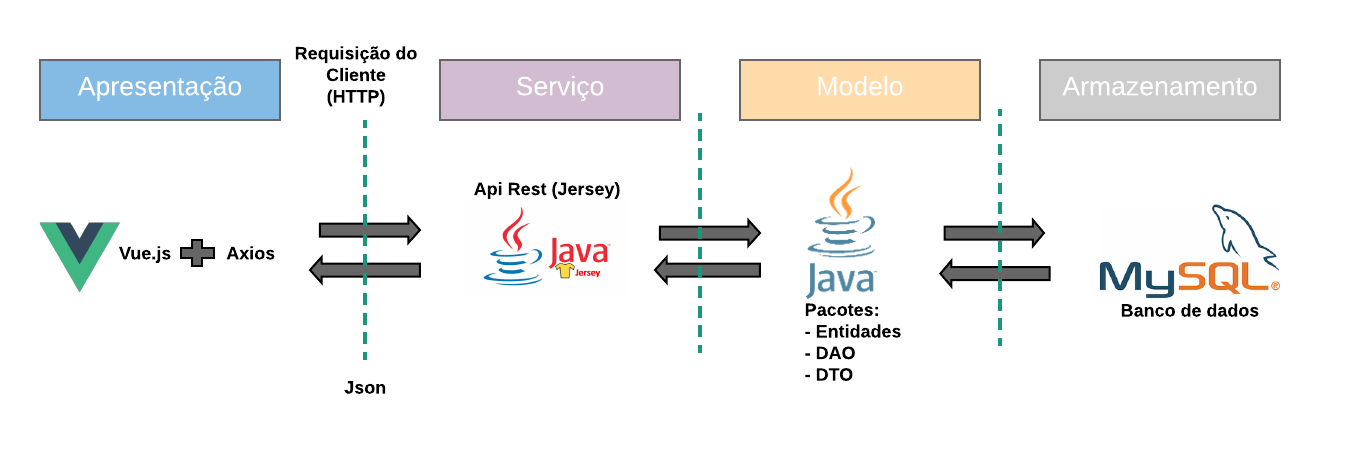
\includegraphics[keepaspectratio=true,scale=0.8]{figuras/arquitetura.png}
	\caption{Representação da arquitetura do sistema.}
	Fonte: {Autor}
	\label{arquitetura}
\end{figure}		

\pagebreak

\subsubsection{Camada 1: Apresentação}
Esta camada envolve todas as tecnologias responsáveis pela apresentação de informações ao usuário e realização de requisições para obter as informações
a serem apresentadas. As principais tecnologias a serem utilizadas para a consolidação desta camada são: HTML, CSS, Vue.js, Axios (requisições) e bootstrap.

\subsubsection{Camada 2: Serviço}
A camada de serviço é responsável pelo preparo e disponibilização de informações obedecendo uma certa estrutura (json para esta proposta de solução) quando estas forem requisitadas. 
Cabe a ela iniciar a comunicação com as subcamadas de forma a solicitar que determinadas informações sejam recuperadas e organizar estas informações em uma estrutura que seja compatível
com o formato de troca de dados estabelecido. Para a construção do serviço, será utilizado o \textit{framework} de construção de APIs REST, Jersey.

\subsubsection{Camada 3: Modelo}
Nesta camada são organizados em pacotes todos os arquivos necessários para realizar o mapeamento de objetos para os tipos de dados aceitos pelo banco de dados
adotado e obter uma conexão com o banco de dados. Esses dois itens citados são feitas por classes DAO (Objeto de Acesso a Dados).

Além das responsabilidades citadas no parágrafo anterior, cabe a esta camada a responsabilidade de definir a estrutura de transferência de dados entre os subsistemas
do software. Este padrão é conhecido como DTO (Objeto de Transferência de Dados) e geralmente são utilizados em conjunto com objetos de negócio de forma a se obter maior
flexibilidade no acesso a determinados dados.

\subsubsubsection{Camada 4: Armazenamento}
Esta camada consiste na utilização de um sistema gerenciador de banco de dados (SGBD), mySql para esta proposta de solução, que passa a ser responsável pelo armazenamento de forma segura e consistente
dos dados do sistema. Além de realizar o armazenamento, o SGB é responsável por recuperar e manipular informações sempre que for necessário e fornece-las sempre que forem solicitadas.

\chapter{Resultados Esperados}
Com os requisitos levantados e priorizados, espera-se que todos eles sejam implementados e integrados ao sistema de forma a fornecer uma boa experiência
de uso. 

Espera-se que a ferramenta seja disponibilizada em um servidor \textit{web} e que este possa ser acessado por todos os alunos interessados em experimentar
a ferramenta.

Ao final do desenvolvimento, é de grande relevância que haja uma quantidade significativa de usuários de forma que se possa levantar informações a respeito
do uso da ferramenta, como por exemplo: sugestões de melhorias, \textit{feedbacks} a respeito da experiência e etc.

Planeja-se aplicar um questionário contendo questões voltadas para o levantamento da experiência obtida pelos jogadores ao utilizarem a ferramenta.

\section{Protótipo}
Ao final do desenvolvimento, espera-se como resultado do \textit{design} do sistema características semelhantes às apresentadas nesta seção. 


\begin{figure}[h]
	\centering
	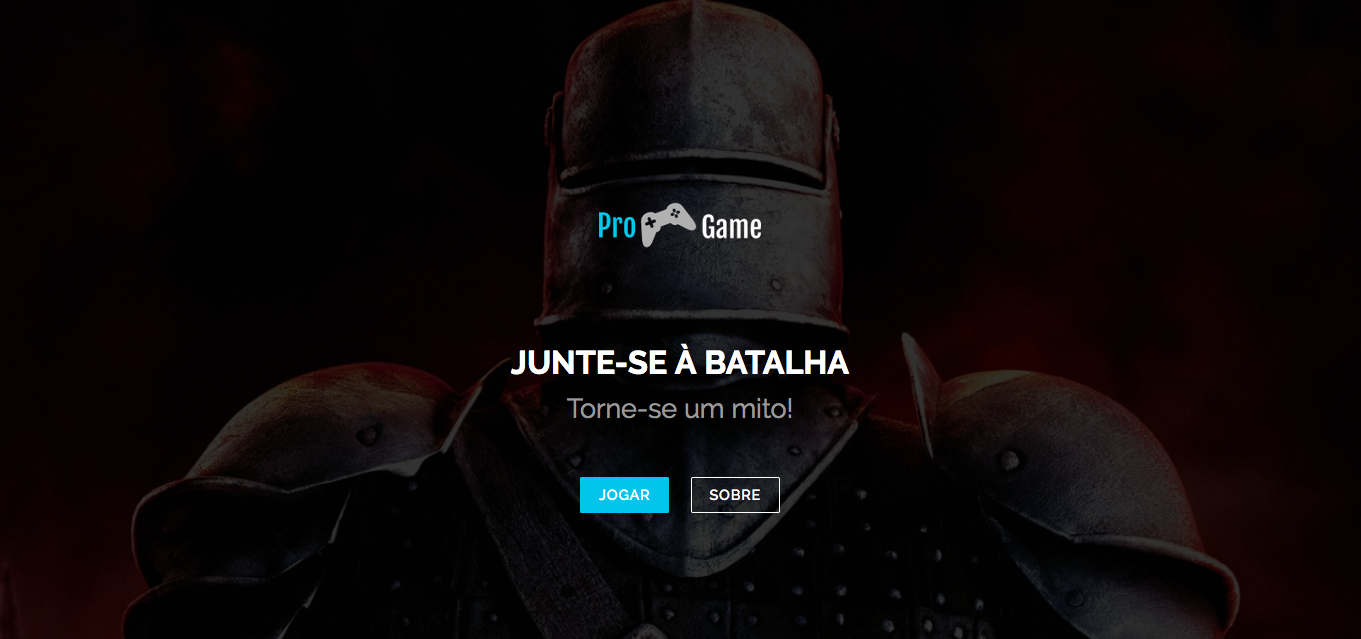
\includegraphics[keepaspectratio=true,scale=0.3]{figuras/inicial.png}
	\caption{Prototipação da tela inicial.}
	Fonte: {Autor}
	\label{telainicial}
\end{figure}	


\begin{figure}[h]
	\centering
	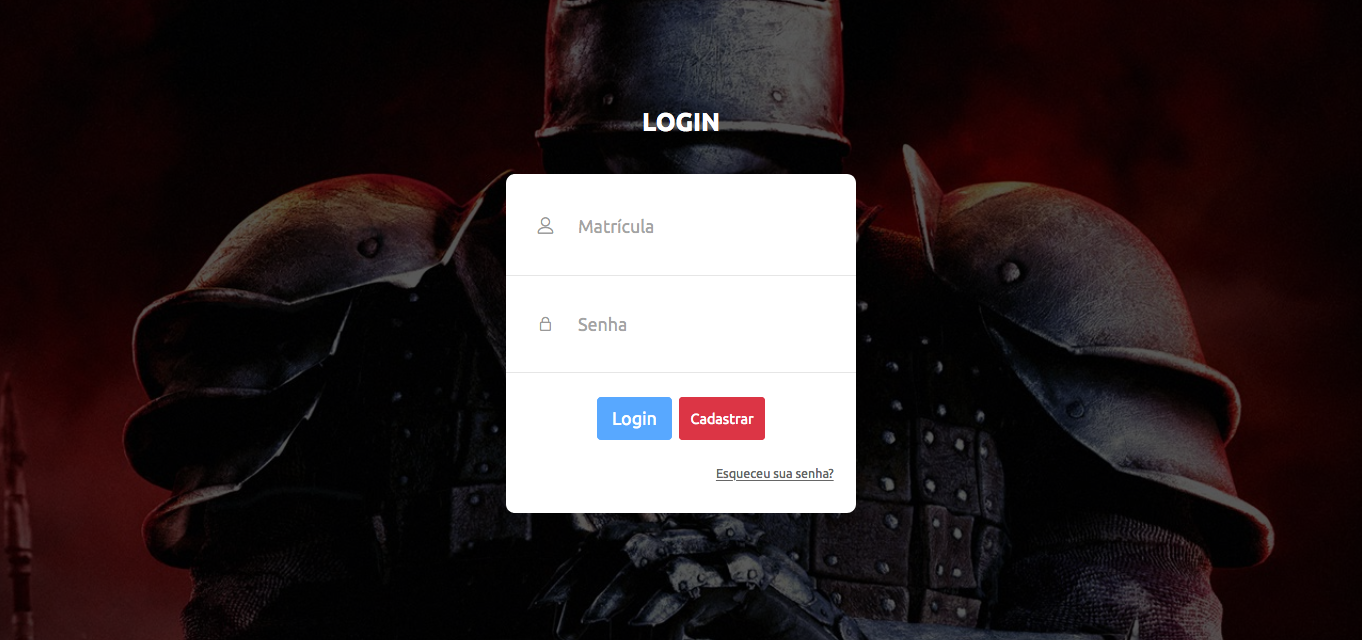
\includegraphics[keepaspectratio=true,scale=0.3]{figuras/login2.png}
	\caption{Prototipação da tela de login.}
	Fonte: {Autor}
	\label{login}
\end{figure}	


\begin{figure}[h]
	\centering
	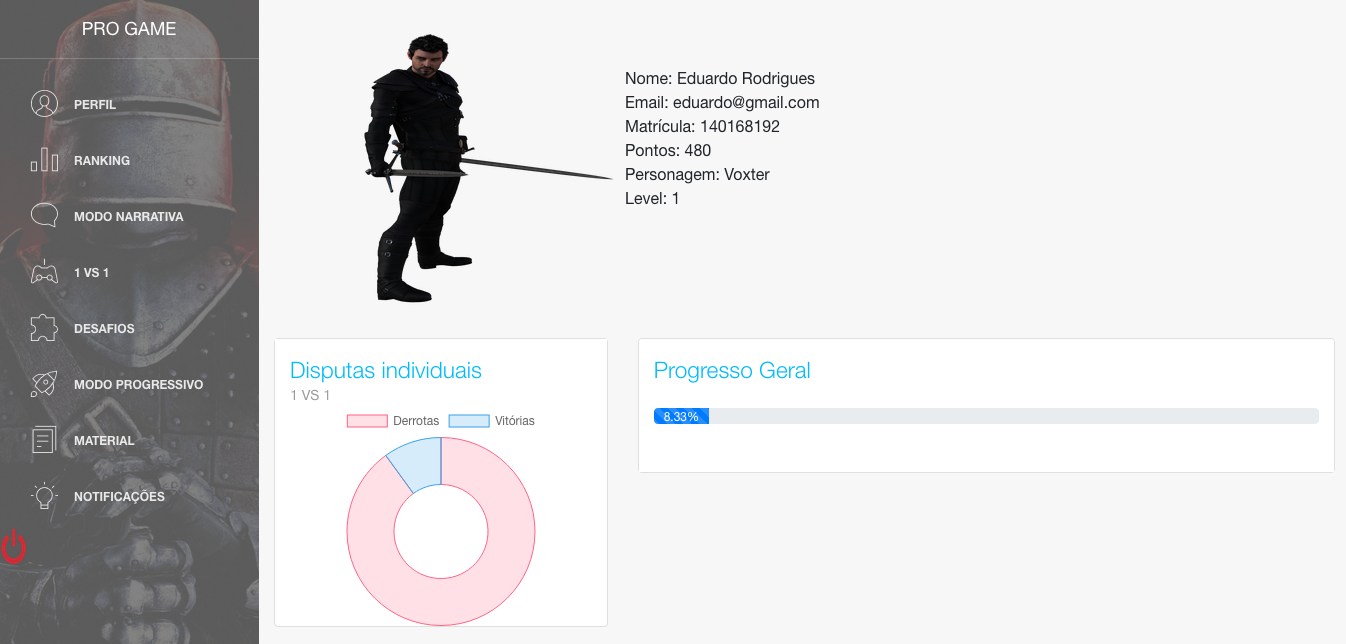
\includegraphics[keepaspectratio=true,scale=0.3]{figuras/perfil2.png}
	\caption{Prototipação menu inicial.}
	Fonte: {Autor}
	\label{menuinicial}
\end{figure}	

\begin{figure}[h]
	\centering
	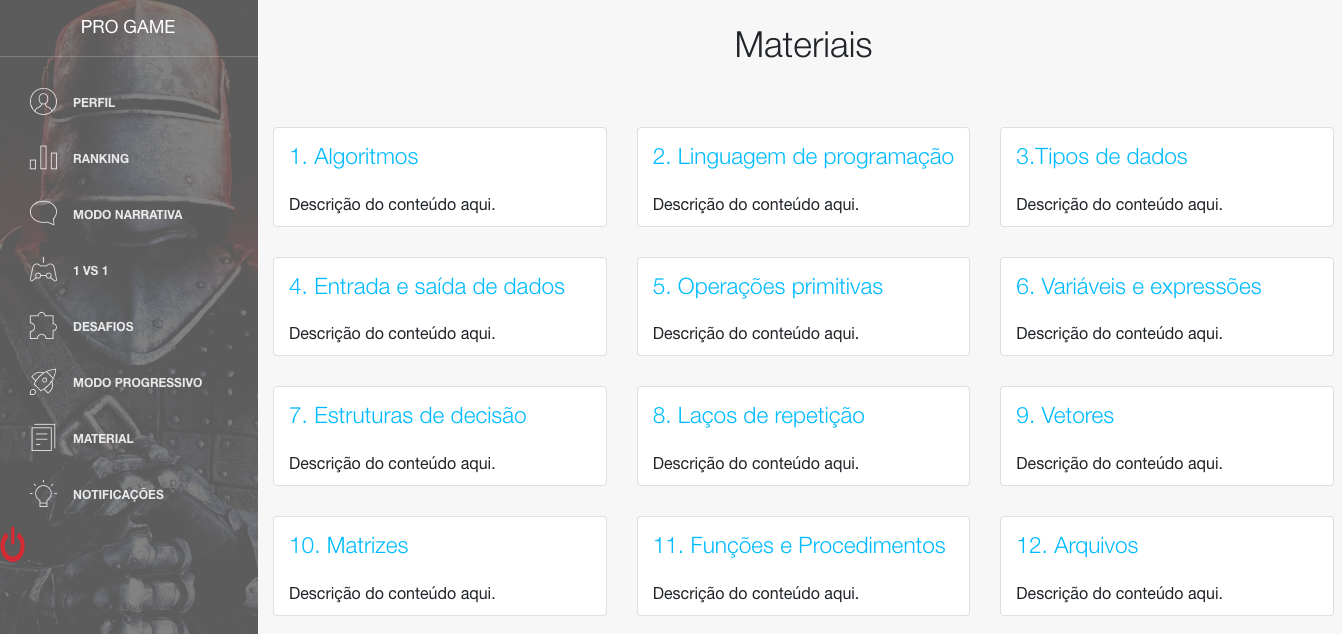
\includegraphics[keepaspectratio=true,scale=0.3]{figuras/material.png}
	\caption{Prototipação módulo material.}
	Fonte: {Autor}
	\label{material}
\end{figure}	

\begin{figure}[h]
	\centering
	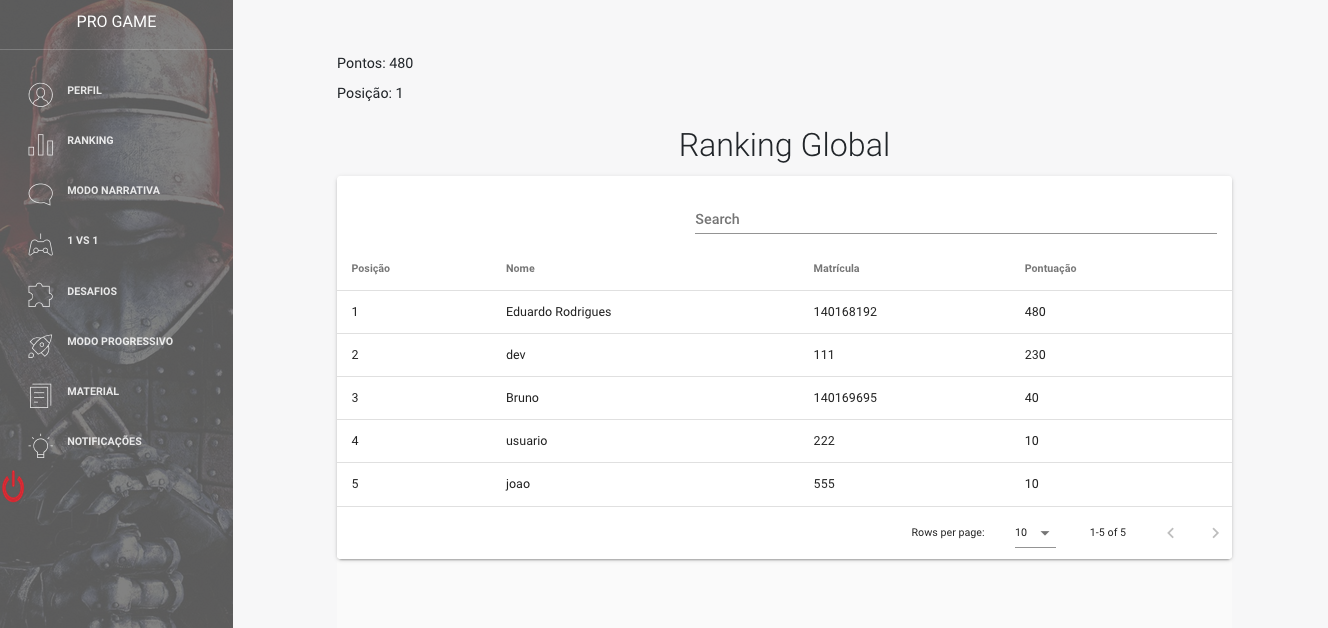
\includegraphics[keepaspectratio=true,scale=0.3]{figuras/ranking.png}
	\caption{Prototipação \textit{ranking}.}
	Fonte: {Autor}
	\label{menuinicial}
\end{figure}	

\begin{figure}[h]
	\centering
	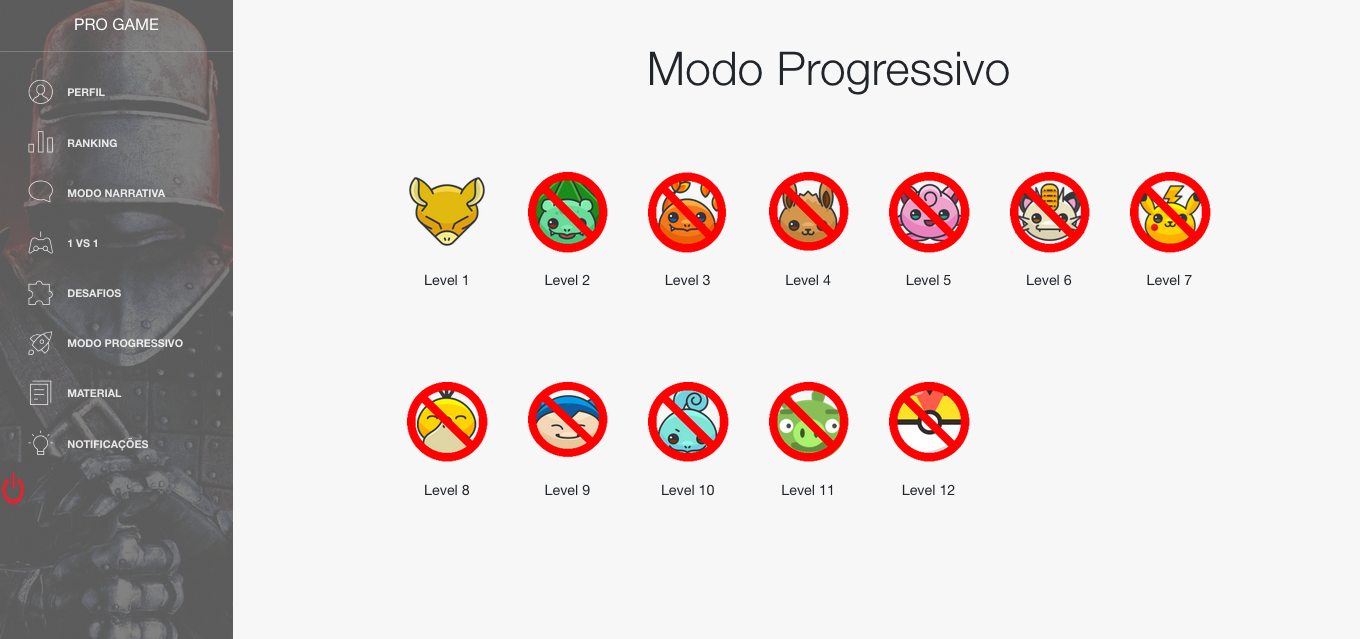
\includegraphics[keepaspectratio=true,scale=0.3]{figuras/progressivo.png}
	\caption{Prototipação menu modo progressivo.}
	Fonte: {Autor}
	\label{material}
\end{figure}	

\begin{figure}[h]
	\centering
	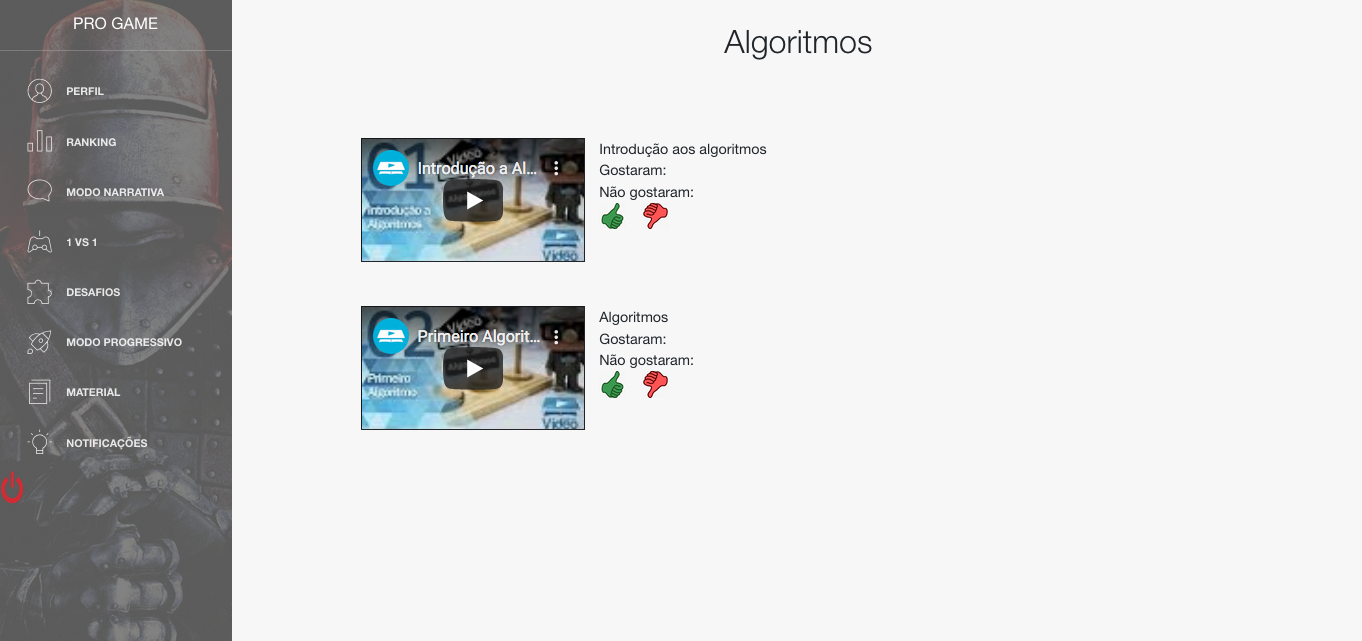
\includegraphics[keepaspectratio=true,scale=0.3]{figuras/materialVideo.png}
	\caption{Prototipação, vídeo aulas do módulo material.}
	Fonte: {Autor}
	\label{material}
\end{figure}	

\chapter{Diferenciais propostos}

Nos capítulos iniciais, foram apresentadas tecnologias com características semelhantes à proposta deste trabalho, porém
algumas características como: materiais/conteúdo de estudo, possibilidade de escolha de personagens temáticos, disputas e desafios entre os jogadores, 
narrativa falada e contextualizada, músicas e sons temáticos entre outras características de jogos que são atraentes aos
usuários, não estão presentes nestas ferramentas e planeja-se desenvolver estas características como uma forma de aumentar o interesse
e engajamento dos usuários.

\chapter{Viabilidade e riscos}
O projeto deve contar com a cooperação de alguns alunos para que se possa realizar um estudo mais direcionado e deve contar com o apoio de alguns professores
para que seja apresentado e seja conhecido pelos alunos. A participação destes dois (alunos e professores) é crítica  e de grande importância para o projeto,
portanto representam um risco para o sucesso deste trabalho.

Além dos riscos apresentados anteriormente, as tecnologias a serem utilizadas não são triviais e requerem um bom conhecimento tanto na arquitetura utilizada
quanto no uso direto de cada uma delas. Mesmo tendo um bom conhecimento nessas tecnlogias, o lançamento de atualizações e descontinuação de algumas delas representam
algum grau de risco para este projeto.

Todas as tecnologias descritas neste trabalho são gratuitas e viáveis de serem utilizadas mas, durante o desenvolvimento pode ser que haja a 
necessidade de uso alguma ferramenta paga, por exemplo a hospedagem da aplicação. Para este cenário serão analisadas os serviços de hospedagem mais
viáveis.

 
\chapter{Cronogramas}
Nas subseções a seguir, são apresentados estimativas de desenvolvimento tanto da proposta de construção da ferramenta (TCC 2) quanto da 
realização dos estudos que justificam e viabilizam a consolidação da proposta (TCC 1). 

É importante ressaltar que os cronogramas apresentados estão sujeitos a mudanças e servem apenas como guia e indicador de progresso.

\section{Cronograma TCC 1}


\begin{table}[h]
	\centering
	\resizebox{\textwidth}{!}{%
	\begin{tabular}{|p{8cm}|p{4cm}|p{4cm}|}
	\hline
	\textbf{Atividade} & \textbf{Data Inicial} & \textbf{Data final} \\ \hline	
		Pesquisa e escrita: Introdução & 05/09/2019 & 10/09/2019 \\ \hline
		Pesquisa e escrita: Referencial Teórico & 10/09/2019 & 30/09/2019 \\ \hline
		Pesquisa e escrita: Metodologia & 30/09/2019 & 25/10/2019 \\ \hline
		Escrita: Resultados esperados & 12/10/2019 & 26/10/2019 \\ \hline
		Escrita: Cronograma TCC 2 & 12/10/2019 & 24/10/2019 \\ \hline
	\end{tabular}%
	}
	\caption{Cronograma TCC 1.}
	\label{perfil}
	Fonte: autor
	% \small{Quadro 1 - Classificação das questões, \citeonline{raposo2016desafio}} 
\end{table}


\section{Cronograma TCC 2}


\begin{table}[h]
	\centering
	\resizebox{\textwidth}{!}{%
	\begin{tabular}{|p{8cm}|p{4cm}|p{4cm}|}
	\hline
	\textbf{Atividade} & \textbf{Data Inicial} & \textbf{Data final} \\ \hline
		Desenvolvimento: Criação da base do projeto de acordo com arquitetura & 22/10/2019 & 22/10/2019 \\ \hline
		Gerência de configuração:  Deploy da base do projeto em um servidor web & 22/10/2019 & 22/10/2019 \\ \hline
		Desenvolvimento  & 12/12/2019 & 20/03/2020 \\ \hline
		Release: Primeira versão do sistema & 20/03/2020 & n/a \\ \hline
		Desenvolvimento & 20/03/2020 & 10/04/2020 \\ \hline
		Release: Segunda versão do sistema & 10/04/2020 & n/a \\ \hline
		Desenvolvimento & 10/04/2020 & 01/05/2020 \\ \hline
		Release: Terceira versão do sistema & 01/05/2020 & n/a \\ \hline
		Desenvolvimento & 01/05/2020 & indefinido \\ \hline
		Questionário de feedback dos usuários: Criação e publicação & 02/05/2020 & 10/05/2020 \\ \hline
		Análise: Resultados e discussão & 10/05/2020 & 10/06/2020 \\ \hline
		Proposta: GCES (Manutenção e evolução do sistema) & n/a & n/a \\ \hline
	\end{tabular}%
	}
	\caption{Cronograma TCC 2}
	\label{perfil}
	Fonte: autor
	% \small{Quadro 1 - Classificação das questões, \citeonline{raposo2016desafio}} 
\end{table}


% \begin{table}[h]
% 	\centering
% 	\resizebox{.8\textwidth}{!}{%
% 	\begin{tabular}{|p{3cm}|p{3cm}|p{8cm}|}
% 	\hline
% 	\textbf{Tecnologia} & \textbf{Frente} & \textbf{Características} \\ \hline
% 	Java & Backend & Linguagem de programação orientada a objetos desenvolvida na década de 90.Diferente das linguagens de programação
% 		modernas que são compiladas para código nativo, a linguagem java é compilada para um \textit{bytecode} que é interpretado por uma máquina
% 		virtual (\textit{java virtual machine}). Por conta disso, a linguagem torna-se altamente portável, isto é, independente de plataforma. \\ \hline
% 	Vue.js & Frontend & \textit{Framework} javaScript voltado para o desenvolvimento de interfaces de usuário.\\ \hline
% 	MySql & Backend & Sistema de gerenciamento de banco de dados que utiliza linguagem sql como interface. Voltado para o armazenamento e manutenção 
% 		de registros de um banco de dados.\\ \hline
% 	Maven & Backend & Ferramenta de automação de compilação muito utilizada em projetos que envolvem a linguagem java. O maven
% 		utiliza um arquivo \textit{xml} (POM) para descrever o projeto de software sendo implementado, suas dependências, componentes
% 		externos, \textit{plugins} necessários, diretórios e ordem de compilação.\\ \hline
% 	Jersey & Backend & \textit{Framework} que facilita o desenvolvimento de APIs (Application Programming Interface) RESTful.\cite{jersey}\\ \hline
% 	Axios & Frontend & bla bla bla bla bla bla bla bla bla bla\\ \hline
% 	JDBC  & Backend & \textit{Driver} que possui um conjunto de classes e interfaces java que permitem o envio/comunicação com qualquer
% 		banco de dados relacional. Permitindo interligar a aplicação com um banco de dados.\cite{jdbc}\\ \hline
% 	Html & Frontend & Linguagem de marcação bastante utilizada na construção de páginas web. Que podem ser interpretados por 
% 		qualquer navegador.\\ \hline \pagebreak
% 	CSS & Frontend & Mecanismo que permite adicionar cores, fontes, espaçamentos e efeitos em um documento \textit{web} (html). \cite{css} \\ \hline
% 	\end{tabular}%
% 	}
% 	\caption{Tecnologias de desenvolvimentos selecionadas}
% 	Fonte: {Autor}
% 	% \small{Quadro 2 - Requisitos funcionais} 
% \end{table}




% \begin{itemize}
% 	\item Levantamento de requisitos (questionários, literatura, ferramentas semelhantes, plano de ensino, currículo pedagógico e etc) -> tabelar
% 	\item Priorização de requisitos (usar o moscow?)
% 	\item Entrevistas (entrevistar colegas que já fizeram e estão fazendo)
% 	\item Conversas com professores
% \end{itemize}

% (frameworks, bibliotecas e etc), documentação da tecnologia entre outros fatores que podem influenciar diretamente
% na construção do sistema.

% Para o desenvolvimento de uma solucão de software, deve-se considerar diversos
% fatores, como: afinidade com as tecnologias de auxílio ao desenvolvimento, recursos disponibilizados pela tecnologia 
% (frameworks, bibliotecas e etc), documentação da tecnologia entre outros fatores que podem influenciar diretamente
% na construção do sistema.

% No desenvolvimento desta ferramenta, a mesma foi dividida em duas áreas principais: backend e frontend. Para cada uma destas
% áreas, apresentamos a seguir as ferramentas utilizadas.


